\documentclass[
%*********************************************
%* Paper type (letterpaper)                  *
%*********************************************
    a4paper,
%   letterpaper,
%   a5paper,
%   b5paper,
%   executivepaper,
%   legalpaper,
%
%*********************************************
%* Font size (10pt)                          *
%*********************************************
%   10pt,
    11pt,
%   12pt,
%
%*********************************************
%* Paging (document dependent)               *
%*********************************************
    oneside,
%   twoside,
%
%*********************************************
%* Equation alignment (center)               *
%*********************************************
%   fleqn,                  %placerer fomlerne i venstre siden istedet for centreret.
%   leqno,                  %Placerer formelnummereringen på venstre side (istedet for højre)
%
%*********************************************
%* Chapter positioning (document dependent)  *
%*********************************************
    openany,                %openany starter chapters på næstkommende side.
%   openright,
%
%*********************************************
%* Language (none)                           *
%*********************************************
%    english]
   danish]
%
%*********************************************
%* Document type (none)                      *
%*********************************************
%   {book}
%   {article}
%   {slides}
    {report}


%*********************************************
%* Userpackages                              *
%*********************************************
\usepackage[latin1]{inputenc} %Bruges til ������
%\usepackage[T1]{fontenc}
\usepackage[danish]{babel}
\usepackage{amsfonts}
\usepackage{mathrsfs}
%\usepackage[xdvi]{epsfig}
%\usepackage{ifthen}
%\usepackage{latexsym}
%\usepackage{theorem}
\usepackage[dvips]{graphicx}       %Used when including .eps (graphics) files
%\usepackage{varioref}
%\usepackage{epic}
%\usepackage{eepic}
%\usepackage{rotfloat}
%\usepackage{multicol}
%\usepackage{wrapfig}
%\usepackage{syntonly}          %Use this to check for proper syntax, makes output file.
%\syntaxonly                %Use this to check for proper syntax, makes NO output file.
\usepackage{verbatim}          %Used when to include an unformatted ASCII file
%\usepackage{fancyhdr}
%\usepackage{layout}
%\usepackage{float}
%\usepackage{makeidx}          %Used when making an index in the document
\usepackage{calc}              %Used if you wanna use cm, mm, ex etc. instead of pt
\usepackage[draft]{fixme}
\usepackage{hyphenat}

\pagestyle
%*********************************************
%* Header / footer configuration (none)      *
%*********************************************
    {plain}                 %Writes page number in footer, header is empty.
%   {headings}
%   {empty}                 %Makes no header or footer
%   {myheadings}
%   {fancy}



%*********************************************
%* Extra pagelayout    (se s. 110)           *
%*********************************************
%\hoffset   =   -0.5cm %Venstremargin
%\voffset   =   0pt
%\evensidemargin=   0pt
%\oddsidemargin =   0pt %Ekstra venstremargin til dobbeltsider
%\topmargin =   -2cm
%\headheight    =   0pt
%\headsep   =   0pt
%\textheight = 690pt
%\textwidth =   480pt
%\marginparsep  =   0pt
%\marginparwidth=   0pt
%\footskip  =   0pt
%\marginparpush =   0pt
%\paperwidth    =   597pt
%\paperheight   =   845pt

%\makeindex

%\parskip   =   1ex
%\parindent =   0em
%\baselineskip  =   2ex

%\underlineheadings

\title{\Huge{}\textbf{Pentominos}\\\Large{}Design dokument\\\vspace{1cm}Dataopsamling p� afd. J p� �rhus Sygehus}
%
\author{Bent Bisballe Nyeng\\deva@aasimon.org\\Aasimon.org}

\newenvironment{apparat}[5]
{
\begin{tabular}{l l}
Apparat:   & #1 \\
Producent: & #2 \\
Form�l:    & #3 \\
Placering: & #4 \\
%Bruger:    & #5 \\
\end{tabular}
}{\\}

%\hyphenation{nøg-le-rings-trans-pon-der}
\hyphenation{Da-ta-ser-ve-ren}
\hyphenation{o-ver-ens}
\hyphenation{ma-ski-ner}
\hyphenation{CPR-ind-tast-nings-me-ka-nis-me}
%\hyphenation{påbe-gynd-e}
%\hyphenation{ef-ter-følg-end-e}
\hyphenation{brug-er-ne}
\hyphenation{for-ma-te-rings-streng}

\markboth{}{}
%*********************************************
%*                start of                   *
%*              -=DOCUMENT=-                 *
%*********************************************
\begin{document}
\maketitle
\tableofcontents

\include{introduktion}
\chapter*{Design m�l}
I projektet er der mange form�l som skal opfyldes, men det er desv�rre
ikke altid muligt at opfylde alle krav samtidig. Derfor er denne
prioriterede liste over designm�lene for integration af procedurer og
apparater udarbejdet:
\begin{enumerate}
\item Fjernelse af alle procedurer som inddrager brugen af papir.
\item Hensigtsm�ssig patientlogistik.
\item Hensigtsm�ssige arbejdsprocedurer.
\item God brugbarhed for dem, som skal betjene udstyret.
\item Forhindring af fejl.
\item H�j systemrobusthed.
\item God ydeevne.
\item Minimering af vedligeholdelsesbyrden.
\item Lave drifts- og anskaffelsesomkostninger.
\item Logning af h�ndelser i systemet.
\end{enumerate}

\noindent Lad os se n�rmere p� de enkelte punkter og bev�ggrundene til deres
prioritering p� listen.

Rette rette rette rette

\section*{1. Fjernelse af alle procedurer som inddrager brugen af papir.}
Da afdelingen netop er blevet p�lagt at arbejde papirl�st, er det en
af topprioriteterne i projektet at fjerne alle procedurer som
bruger eller producerer data p� papir.

\section*{2. Hensigtsm�ssig patientlogistik.}
Der vil blive �ndret p� arbejdsprocedurerne mange steder p� afdelingen.
Af hensyn til patienterne er det derfor vigtigt at holde fokus p�
deres logistik i disse �ndringer.

Eftersom vi mange steder p� afdelingen kommer til at �ndre meget p�
arbejdsprocedurerne er det vigtigt at der blivar sat stor fokus p�
hvordan patienterne kommer til at m�rke disse �ndringer, og at de
kommer til at opleve det som en forbedring, eller slet ikke.

\section*{3. Hensigtsm�ssige arbejdsprocedurer.}
For personalet p� afdelingen er det ligeledes vigtigt at
arbejdsprocedurer bliver lavet p� en hensigsm�ssig m�de, s� der ikke
bliver introduceret uhensigsm�ssigheder for de ansatte i forbindelse
med de nye procedurer.

\section*{4. God brugbarhed for dem, som skal betjene udstyret.}
Det skal v�re intuitivt nemt at forst� hvordan udstyret skal betjenes
s� det ikke kr�ver en lang introduktion, inden brugerne kan benytte
systemerne med fuldt udbytte.

\section*{5. Forhindring af fejl.}
Systemerne skal desgines s� det i s� lang udstr�kning som det er
muligt kan forhindre at der sker fejl.

\section*{6. H�j systemrobusthed.}
Systerne skal designes s� de er fejltollerante, dvs. de skal ikke
blive ustabile eller holde op med fungere fordi dets omgivelser ikke
opf�rer sig korrekt eller som forventet.

\section*{7. God ydeevne.}
Systemerne skal designes s� de ikke sl�ver arbejdsgangen. Alle svartider
skal v�re sm� s� brugerne ikke bliver ut�lmodige og systemerne skal
v�re interaktive og responsive under brugen.

\section*{8. Minimering af vedligeholdelsesbyrden}
Systemerne skal desgines s�dan at de er nemme at vedligeholde,
udskifte eller udbygge, s� det ikke kommer til at kr�ve ret meget
arbejde fra det tekniske personale.

\section*{9. Lave drifts- og anskaffelsesomkostninger.}
Systemerne skal v�re s� billige som muligt i anskaffelse, s� de ikke
bliver en stor �konomisk byrde for afdeligen, hvilket i s� fald ville
medf�re en l�ngere udruldningstid.

\section*{10. Logning af h�ndelser i systemet.}
Alle systemer skal lagre alle udf�rte delopgaver et let tilg�ngeligt
sted p� en m�de som er l�sbar af mennesker. Dette skal g�res for at
sikre gode muligheder for trackning af h�ndelser i systemet uden at
man rent faktisk skal bringe dette ud af drift eller p� lingende vis
p�virke den daglige drift.

\fixme{Afrunding / konklusion}

\part{Observationer} % Hvad har vi
\chapter{Udstyr}

\fixme{introduktion/indledning}


\fixme{L�g generelt v�gt p� patientens forl�b ogs�, istedet for kun l�gens}
%Der er to typer udstyr i vores system, det som producerer data, og det
%som transporterer og lagrer data.\\
%Den f�rste type har vi meget lidt eller slet ingen kontrol over, men
%m� her l�ne os op ad de specifikationer som producenterne stiller
%til r�dighed.
\section{Apparatur}
\fixme{Tabellen skal krydcheckes mht. apparatnavne}
\begin{figure}
\begin{center}
\begin{tabular}{|l|c|c|c|c|}
\hline
Apparat                  & Push & Pull & Manuel & CPR-Aware\\
\hline
\hline
Lensometer               & X    &      & X      &      \\\hline
Keratometer              &      & X    & X      &      \\\hline
Tonometer                &      & X    & X      &      \\\hline
Retinometer              & X    &      & X      &      \\\hline
Phoropter                & X    &      & X      &      \\\hline
Spaltelampe              & G    &      &        &      \\\hline
Diktafon                 &      & X    &        &      \\\hline
ACMMaster                & S    &      &        & X    \\\hline
IOLMaster                & X    &      &        & X    \\\hline
Ophthasonic              &      &      & X      &      \\\hline
A4 Scanner               & X    & X    &        &      \\\hline
%SortSmartKasse           & ?    & ?    &        &      \\\hline
Atlas                    & S    & ?    &        & X    \\\hline
Pupilometer              & S    &      &        & X    \\\hline
Wasca                    & S    &      &        & ?    \\\hline
Keratometer NRK8000      & X    &      &        & X    \\\hline
Digatal Foto Kamera      & ?    & ?    &        &      \\\hline
Ultrasound Biomicroscope &      &      &        &      \\\hline
PC-Praxis                & S    & S    &        & X    \\\hline
Field Analyzer           & X    &      &        & X    \\\hline
Laser 'argon'            & ?    & ?    &        &      \\\hline
SmartLens                & ?    & ?    &        &      \\\hline
Stratus OCT              & S    &      &        & X    \\\hline
SLO101                   & G    &      &        &      \\\hline
Fundus Kamera            &      & X    &        &      \\\hline
Barcode reader           &      & X    &        & X    \\\hline
OP Microskop             &      & G    &        & X    \\\hline
Alcon Infinite           & ?    & ?    &        &      \\\hline
YAG laser OP3            & ?    & ?    &        &      \\\hline
Ophthalas 532 eyelite    & ?    & ?    &        &      \\\hline
Cryostar                 &      &      &        &      \\\hline
Mel 80                   & ?    & ?    &        & ?    \\\hline
LSK Evolution2           &      &      &        &      \\\hline
AL100 Biometer           & ?    & ?    &        &      \\\hline
Blodtryksm�ler           & ?    & ?    & ?      & ?    \\\hline
\end{tabular}
\end{center}
\label{app}
\caption{Tabellen viser alle de apparater p� afdelingen som er relevante i
	forbindelse med opkobling.'X' betyder, at denne egenskab er til
	stede. 'G' betyder, at denne egenskab er til stede vha. af et
	grabber program (a la PC-Grab). 'S'	betyder, at der kan uploades
	filer til et samba drev, og '?' betyder, at det ikke vides om denne
	egenskab er til stede.}
\end{figure}

P� figur \ref{app} ses en liste over alle de apparater p� afdeligen, som er
relevante i opkoblingsprocessen.\\
Apparats�jlen beskriver hvilket apparat, der er tale om, Pushs�jlen
fort�ller om apparatet kan pushe data ud n�r det produceres, Pulls�jlen
fort�ller om man udefra kan sp�rge apparatet om dets data for at f�
dem, Manuels�jlen fort�ller om apparatet kan printe en lap papir ud med dets
data, og CPR-Awares�jlen fort�ller om apparatet har nogen ide om, hvilken
patient det er i gang med at producere data til.
\fixme{Der mangler et afsnit som binder apparater og arkitektur sammen.}

\section{Computere}
Der findes fire typer computere i systemet:
\begin{enumerate}
\item Serveren
\item Soekris bokse \fixme{Find p� nogt abstrakt at kalde
  Soekrisboksene p� dette stadie}
\item Tykke klienter (f.eks MIaV og Fundus)
\item Klient maskiner
\end{enumerate}
\fixme{Uddyb}
\noindent Serveren er der kun een af og den binder det hele sammen via
to netv�rk. Soekris boksene er der mange af, og de er koblet op mod
serveren for at levere data til den (read-append). De tykke klienter har umiddelbart
samme rolle som Soekrisboksene, men indeholder v�sentligt mere
kompliceret software, som i sig selv laver databehandling udover
leveringen af data til serveren (read-append). Klienterne er alle de maskiner p�
afdelingen, som har behov for at udtr�kke data fra serveren (read-only).

\begin{figure}
\begin{center}
\includegraphics[width=120mm]{udstyr.eps}\\
\end{center}
\label{udstyr}
\caption{Computerne i projektet. Pilene indikerer datatransport. De
	stiplede bobler indikerer de isolerede netv�rk.}
\end{figure}

\section{Lokationer}
\fixme{Mere om patienterne}
Der vil blive defineret nogle logistiske lokationer, som har en
arbejdsm�ssig sammenh�ng. Det kan v�re et lokale, eller en afgr�nset
samling af maskiner og/eller apparatur.\\
Hver lokation bliver knyttet sammen af en central
CPR-indtastningsmekanisme, som har til form�l at levere det CPR-nummer,
som dataene fra apparaturet p� lokationen skal lagres under.\\
Flere lokationer er s�ledes selvdefinerende (f.eks en operationsstue),
mens andre er mere spidsfindige at definere (f.eks det store
unders�gelsesrum ved siden af kateraktsporene).\\
Der skal s� vidt muligt s�rges for, at to patienter ikke kan
behandles i den samme lokation samtidig, hvilket effektivt betyder, at
vi i mange tilf�lde er n�dt til at definere en lokation som et
enkelt apparat.\\

\section{Brugerregistrering}
For at kunne registrere hvilken bruger, som har til hensigt at foretage
en m�ling, er det n�dvendigt med en form for registrering f�r
begyndelsen af m�lingerne.\\
Dette kan g�res vha. af gammeldags login/password, hvilket er
besv�rligt at udf�re, specielt hvis det skal ske mange gange
dagligt. Endvidere kan det ske vha. af en form for stregkode eller
magnetkort, som brugerne skal have p� sig, mens de befinder sig p�
afdelingen. Disse er hurtigere at benytte, men har den ulempe, at de er
skr�belige, specielt ved hyppigt brug. Den sidste og umiddelbart
bedste l�sning er indf�relsen af s�kaldte RFID tags, som fungerer p� den m�de,
at brugeren skal vifte tagget (som kan have vilk�rlig udformning og
st�rrelse) foran en plade. De er meget billige at anskaffe og er meget
robuste, kan s�gar t�le grundig vask med sprit eller en tur i 
t�rretumbleren, hvilket l�ser en del af de hygiejneproblemer som m�tte
forekomme i de to andre l�sninger.\\
\fixme{Duer ikke med \LaTeX{} handsker - desuden kr�ves registrering af
  personf�lsom data for l�gerne = skidt}
Fingeraftryksl�ser har ogs� v�ret p� tale, men eftersom denne
teknologi giver en r�kke hygiejneproblemer, samt at den endnu ikke er
100\% p�lidelig, er den ikke anbefalelsesv�rdig til dette projekt.\\
For at kunne indl�se og sende brugerkoden til dataserveren skal
flg. udstyr s�ledes opstilles p� hver lokation:
\begin{itemize}
\item RFID l�ser.
\item Soekris boks med PoE udstyr.% adapter (Power over Ethernet).
\end{itemize}
Det overvejes at alle brugerne skal have et kort eller lignende med
indbygget RFID tag, som de skal inds�tte i en spr�kke og lade sidde i
denne spr�kke, s� l�nge unders�gelsen eller operationen er i
gang. Systemet kan p� denne m�de hele tiden vide, hvilken bruger, der betjener
systemet, og samtidig slipper man for problemer som opst�r fordi en bruger
glemmer at aktiverer sit tag (logge ind) i systemet inden en
unders�gelse, hvilket vil give nogle problemer som ikke er mulige at
opdage ved systemcheck. Hvis en bruger har glemt sit tag ved en
tidligere unders�gelse, kan den n�ste ikke foretages, hvorved brugeren
tvinges til at holde sit tag p� sig under hele arbejdsdagen.\\
Hvis en bruger har mistet sit tag, skal der laves fallbackl�sninger, s�
det er muligt at f� et midlertidigt tag, som kan redirigere systemet til den
p�g�ldende bruger internt.

\begin{figure}
\begin{center}
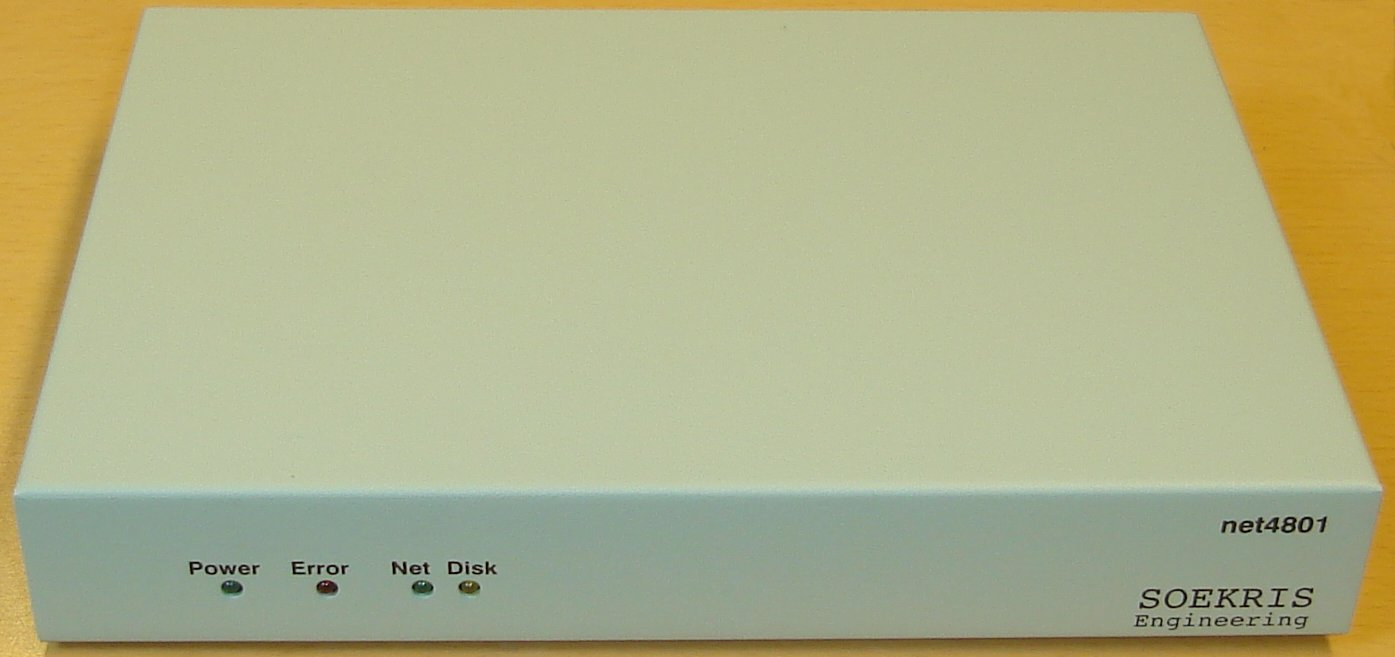
\includegraphics[width=60mm]{soekris_front.eps}
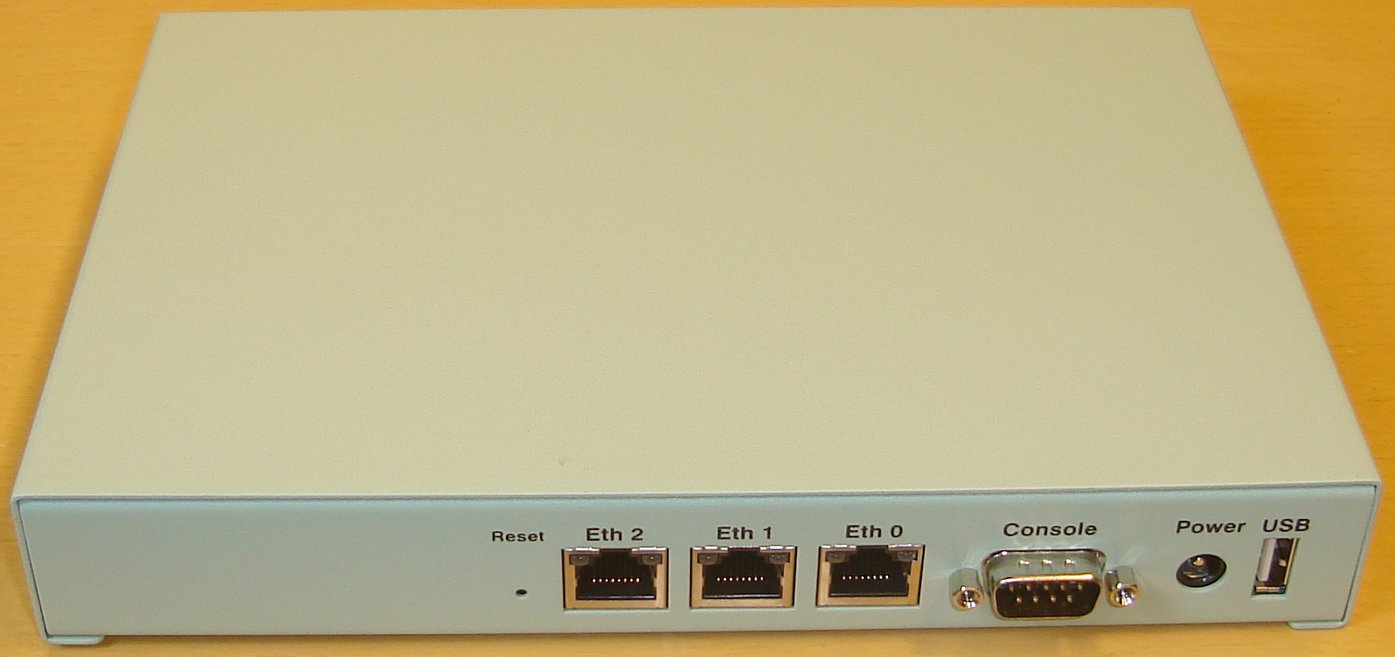
\includegraphics[width=60mm]{soekris_back.eps}\\
\end{center}
\label{soekris}
\caption{Soekrisboksen set forfra og bagfra.}
\end{figure}

\section{CPR-indtastning og dataopsamling}
For at kunne levere et CPR-nummer skal flg. udstyr stilles til
r�dighed for hver lokation:
\begin{itemize}
\item Nummerisk tastatur.
\item Sygesikringskortl�ser.
\item Soekris boks (gerne fysisk den samme, som den der skal l�se RFID tags).
\end{itemize}
Soekris boksen skal via serielkabler, USBkabler eller lignende v�re koblet fysisk til
alle apparaterne i lokationen og derved fungere som opsamlingspunkt
for dataene. N�r et CPR-nummer indtastes (eller magnetkort l�ses)
bliver det knyttet til det givne lokationsnummer (her kan lokalenummer
+ eventuelt underkode benyttes). Soekris boksen opsamler dataene og
videresender dem r�t til dataserveren sammen med
lokationsnummeret. Dataserveren er samtidig blevet gjort opm�rksom p�
hvilket CPR-nummer, som h�rer til det p�g�ldende lokationsnummer, og ved
derfor, hvor i databasen den skal lagre dataene.\\
Dataene bliver p� intet tidspunkt fortolket -- dette sker f�rst n�r
dataene skal l�ses ud igen.\\
Der er intet til hinder for at der kobles flere Soekris bokse p� en
lokation, idet CPR-nummeret ikke er boks specifikt, men lagres globalt
p� dataserveren.\\
Hvis en patient har glemt sit sygesikringbevis eller magnetstriben er
beskadiget er det muligt at indtaste CPR-nummeret manuelt, men
eftersom dette er besv�rligt og potentielt fejlproducerende (der tastes
forkert), skal der ved ankomsten laves et system, hvor patienten f�r
et 'erstatnings sygesikringsbevis' som indeholder en speciel kode,
som i systemet s�ttes til at referere til et konkret CPR-nummer. Det
samme system kan bruges ved patienter uden CPR-nummer, eller ved
patienter med erstatningsnumre.\\
En funktion i administrationssoftwaren skal, for at f� fuldt udbytte
af denne funktionalitet, kunne udskifte et givent CPR-nummer med et
andet (F.eks. hvis en nyf�dt behandles, f�r der er tildelt et
CPR-nummer. Her vil unders�gelsen foreg� under et erstatsningsnummer,
men en uge senere skal de m�lte data flyttes til det faktiske
CPR-nummer, n�r den nyf�dte har modtaget dette.).

\begin{figure}
\begin{center}
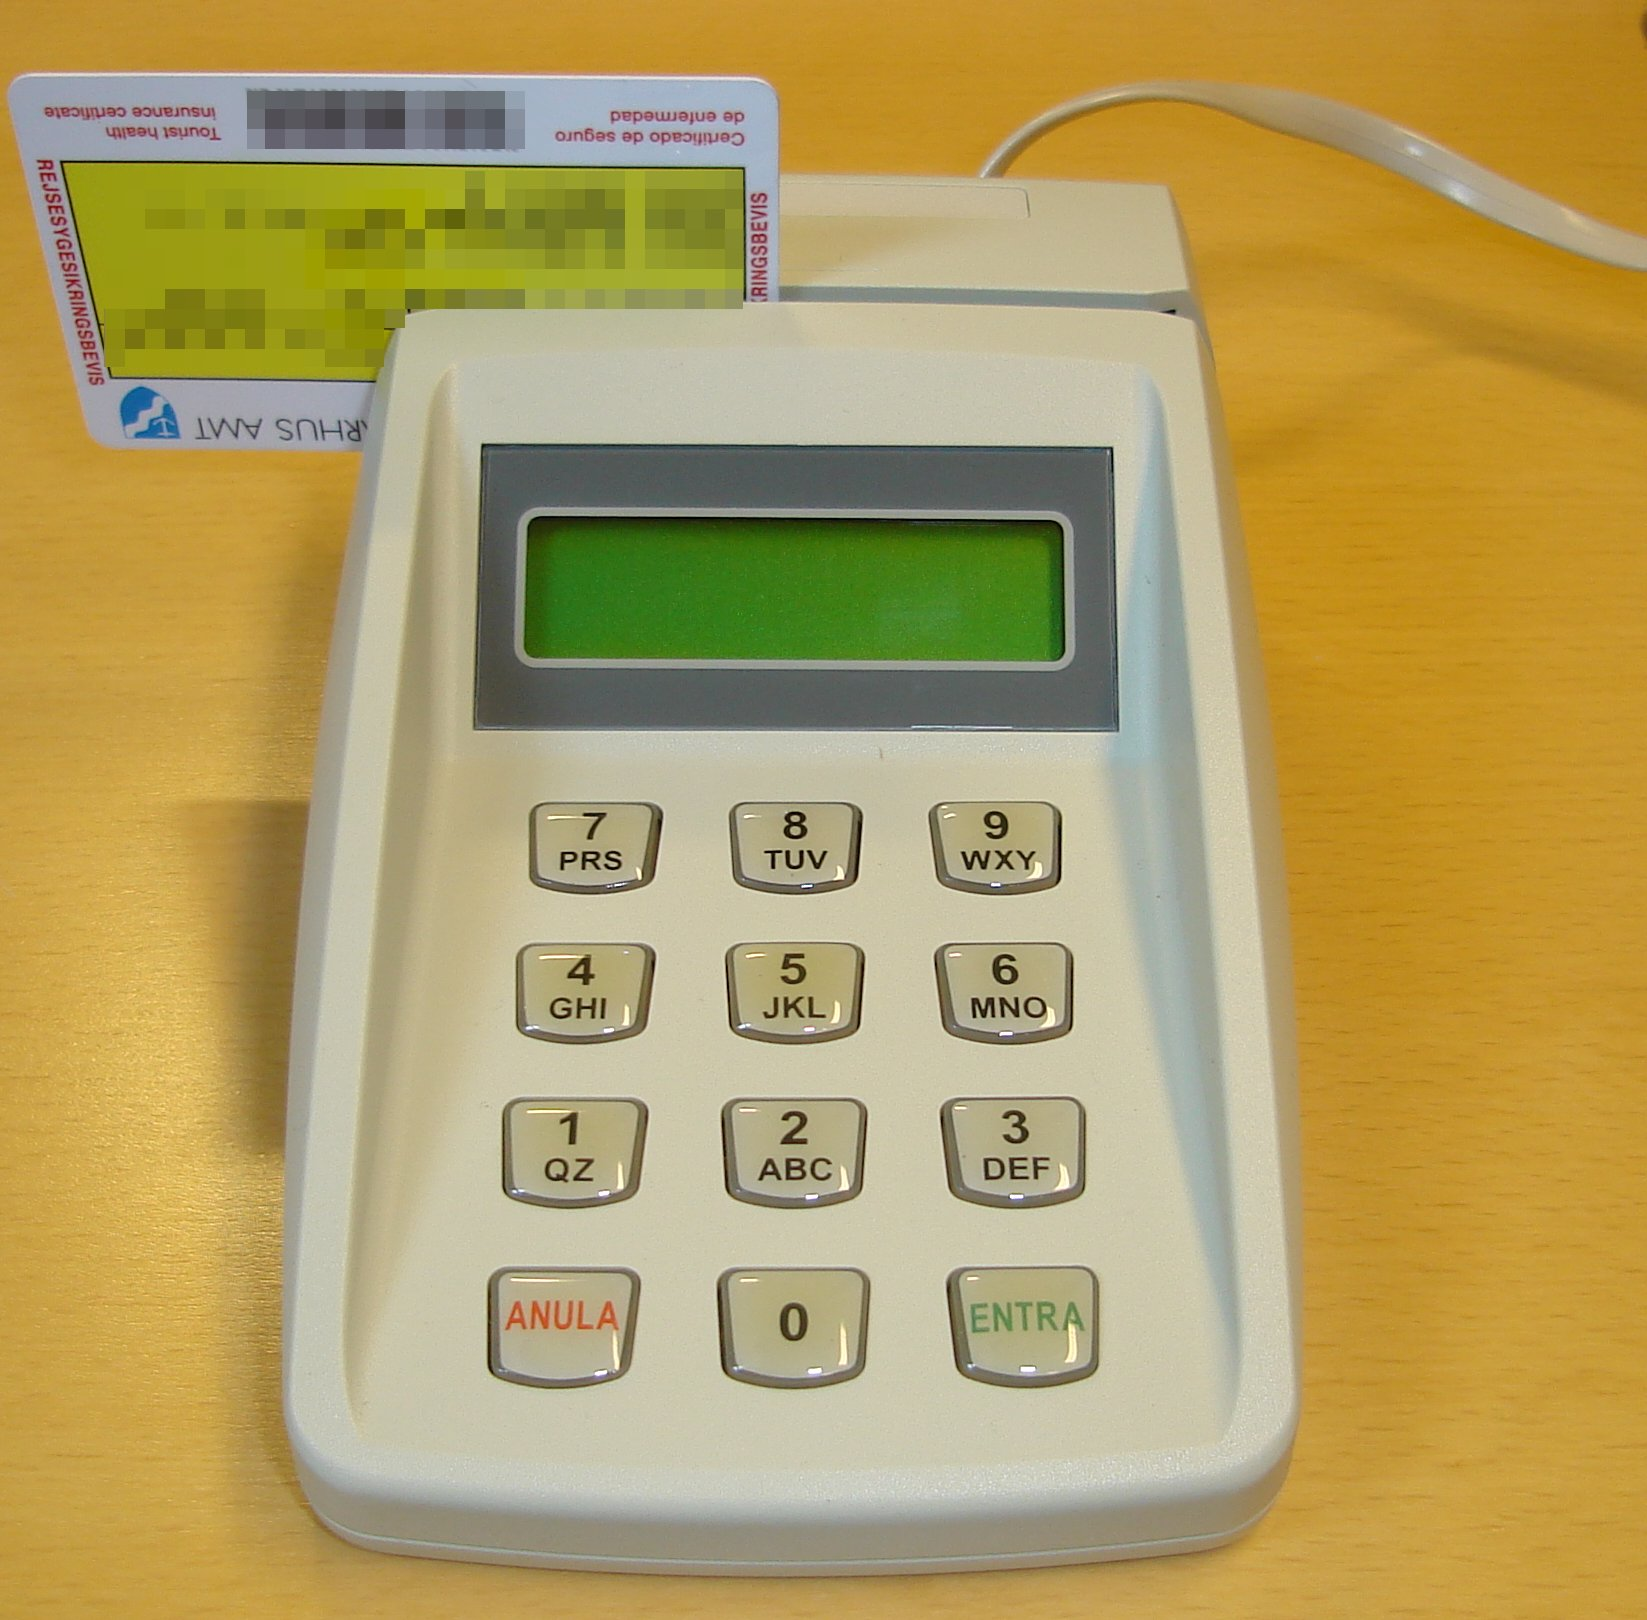
\includegraphics[width=80mm]{cpr_tastatur.eps}\\
\end{center}
\label{cpr}
\caption{CPR tastatur med indbygget magnetkortl�ser og display.}
\end{figure}

\section{Dataudl�sning}
Det lagrede data er gemt r�t med henblik p� at bevare kontinuiteten i
dem (hvis vi beslutter, at vi vil gemme en vis delm�ngde af dataene,
kan vi en dag f� brug for mere - p� denne m�de lagres alting altid).\\
N�r en applikation �nsker at bruge data fra et apparat, kontakter det
dataserveren med et CPR-nummer og en apparatkode, samt en
formateringsstreng. Dataserveren kan nu l�se de r� data fra databasen
og lave en fortolkning, som stemmer overens med den formateringsstreng,
som klienten har vedh�ftet foresp�rgslen. Herefter kan dataserveren
svare p� foresp�rgslen p� en m�de, som er veldefineret for
klienten. Disse formateringsstrenge specificerer vi dynamisk,
efterh�nden som nyt apparatur og nye klienter tilknyttes systemet.

\section{Implementation}
Grundet den dynamiske og skal\'{e}rbare opbygning af systemet kan vi
p�begynde tilslutningen og brugen allerede n�r CPR-udstyret er
lavet.\\
Soekris boksene skal have ens konfiguration s� man nemt og hurtigt kan
skifte en defekt boks ud med en anden, uden tab af funktionalitet.\\
Ydermere skal deres filsystem opbevares centralt, eventuelt p�
dataserveren, s� opdateringer af software og lignende kan ske centralt og
ikke pr. boks.\\
Dette vil selvf�lgelig medf�re \textit{single point of failure} idet alle boksene vil
v�re inaktive ved en fejl p� dataserveren. Men eftersom Soekris
boksene er afh�ngige af dataserveren for at kunne sende data, �ndrer
det ikke noget, hvis de selv opbevarede deres filsystemer, idet de stadig
ikke ville kunne sende data (og dermed fungere korrekt), hvis
dataserveren var nede.

\section{Bagudkompatibilitet}
Da der findes en lang r�kke systemer p� afdelingen, som kommer til at
v�re i brug l�nge efter dette system bliver sat i drift, er det
vigtigt, at det nye system er i stand til at samarbejde med de
eksisterende, uden at der g�es p� kompromis med funktionalitet og
design af det nye system.\\
Konkret drejer det sig om PC-Praxis og registrering af m�ledata, samt
arkivering af billeder til senere visning i PC-Show.\\
Det p�t�nkes at lave et VFS-modul til sambaserveren, som kan
registrere data korrekt til senere l�sning i PC-Praxis. Det fungerer
p� den m�de at alle kald til sambaserveren hookes og overrides af det
som dikteres af VFS modulet, hvilket s�rger for at alle filoverf�rsler
kan laves indirekte i en database eller i en filstruktur, som vi har
fuld kontrol over. VFS modulet skal s�ledes til en vis grad overs�tte
PC-Praxis journal requests til faktiske databaseopslag.\\
Hvorvidt denne strategi vil virke i praksis vil vise sig efter en r�kke
praktiske afpr�vninger.

\fixme{afrunding/konklusion}

\part{Analyse} % Hvad vil vi gerne have
\chapter{Arbejdsprocedurer}
\fixme{Skidt indledning}
I dette kapitel vil det blive belyst hvilke typer arbejdsopgaver som
typisk forekommer p� afdeligen. Samtidig vil det blive belyst hvilke
typer apparatur der findes, samt hvordan en bestemt type apparatur
er med til at diktere den nuv�rende arbejdsprocedure.\\
Alt dette vil blive belyst ved en r�kke passive observationer af
faktiske arbejdssituationer med faktiske patienter, hvilket burde
give anledning til de mest korrekte beskrivelser, modsat f.eks hvis
brugerne blot var blevet bedt om at beskrive deres egen arbejdsprocedure,
hvorved de typisk vil glemme at fort�lle de operationer som for dem er
�benlyse og trivielle, men potentielt kritiske for det fremtidige
design af systemet.

\section{Analyse}
\fixme{Hvad vil vi have, hvad har vi, hvad skal laves om og hvad mangler}
N�r man ser generelt p� disse observationer, bliver det klart, at
procedurerne styres af apparaterne, og ikke omvendt, hvilket i mange
tilf�lde medf�rer uhensigtsm�ssige procedurer, som i v�rste fald kan
medf�re fejl.\\
Hvis man kigger p� konkrete apparater og deres procedurer er der klart
nogle der er v�rre end andre.\\
Blandt de v�rste kan n�vnes pupilometeret, hvor arbejdsgangen tvinger
brugeren til at producere data, som ikke senere skal benyttes.\\
Nogle apparater producerer udelukkende resultaterne p� en
sk�rm, hvor brugeren skal l�se dem og manuelt indtaste dem i et andet
system. Det er uhensigtsm�ssigt, idet der s�ledes skal skiftes
mellem applikationer og/eller computer, hvilket leder til �get risiko
for fejl.\\
Andre apparater producerer resultaterne p� en papirstrimmel som
efterf�lgende skal indtastes manuelt eller indscannes p� en A4
scanner.\\
Der er dog ogs� apparater, som dikterer en hensigtsm�ssig procedure,
deriblandt de apparater, som er koblet direkte p� PC-Praxis
(tonometer, keratometer). Dette afspejler dybest set den
funktionalitet, som �nskes skal v�re til stede p� alle apparater p�
afdelingen. Den direkte integration er dog begr�nset til PC-Praxis og
nogle udvalgte apparater, hvilket g�r det problematisk blot at
udvide den model til alle apparaterne.\\

De v�rste arbejdsgange er dem, hvor brugerens handlinger er dikteret af
apparatet p� en m�de, som er uhensigsm�ssig i forhold til
patientkontakt. Det g�lder f.eks hvis en l�ge er tvunget til at vende
ryggen til sin patient, eller m�ske endda forlade lokalet i nogle
minutter, som det er tilf�ldet ved IOL Masteren hvor brugeren m� bev�ge
sig ud af lokalet for at indscanne en printet graf.\\
Arbejdsgange som kr�ver manuel indtastning er ligeledes slemme, idet
de introducerer stort potentiale for fejl, i form af d�rlig hukommelse
hos brugeren, eller generel uopm�rksomhed, hvilket kan lede til
fejlindtastede v�rdier. Dette kan igen p� sigt medf�re forkerte
resultater og i v�rste fald (hvis ikke fejlene bliver fanget) en
forkert forl�bskonklusion.
\chapter{Brugbarhed}
Det er vigtigt at systemerne er nemme at benytte for brugerne, s� man
undg�r fejl, der opst�r pga. af forkert betjening. Eftersom
systemet vil blive benyttet adskillige gange dagligt af de samme
mennesker, er det dog samtidig vigtigt at denne let-tilg�ngelighed ikke
bliver en byrde for brugerne, s� de bliver tr�tte af at bruge systemet.\\
Det endelige brugbarheds princip er derfor at systemerne skal v�re
responsive og informative, men p� en ikkeforstyrrende m�de.\\
Det skal signaleres til brugeren, n�r data er sendt afsted og korrekt
modtaget p� en m�de som ikke generer arbejdsgangen og patienterne, og
samtidig uden at brugeren skal flytte sig, trykke p� noget eller p�
lignende vis aktivt g�re en indsats for at f� statusmeldinger.\\
Det kan f.eks. implementeres vha. af diskrete bippelyde, p� samme m�de
som det kendes fra supermarkedets kassesystem. Ved apparater, hvor
brugeren ser p� en sk�rm under produktionen af dataene, kan systemet
informere vha. lysdioder eller lign. monteret omkring sk�rmen, indenfor
synsvidde.\\
Udover denne umiddelbare respons skal der samtidig v�re mulighed for
at se status p� handlingen, hvis brugeren af een eller anden grund
skulle blive i tvivl om, hvorvidt den handling, der netop er foretaget,
rent faktisk var den forventede, alts� en form for visuel historik.\\
Et eksempel kan v�re, at en bruger har indtastet et CPR-nummer og
foretaget en m�ling p� et apparat, hvorefter brugeren bliver
i tvivl om, hvorvidt det rent faktisk var det rigtige CPR-nummer, der
blev sendt med. Her skal det kunne ses p� et display, at dataene er
korrekt modtaget p� serveren, samt hvilket CPR-nummer de er blevet knyttet til
i databasen, s� brugeren kan konstatere, om det er det rigtige.\\
En vigtig pointe med udarbejdelsen af de nye arbejdsprocedurer er, at
brugerne maksimalt g�r det samme som de g�r i \hyphenation{for-vej-en}forvejen - vi vil
s�ledes kun fjerne elementer fra arbejdsgangen eller erstatte
eksisterende elementer med nye, tilsvarende elementer. Det er
ekstremt vigtigt for oplevelsen af systemet, at brugerne opfatter det
som en forbedring i forhold til det, de havde i forvejen. For�get
funktionalitet som ikke er synlig for brugeren, s�som logning af
h�ndelser, m� s�ledes ikke blive introduceret p� bekostning af
arbejdsgangen.
\chapter{Forhindring af fejl}
%Da det er af meget stor vigtighed, at der ikke opst�r fejl i
%dataoverf�rsler, skal der indf�res en r�kke procedurer for at
%forhindre at dette sker.\\
Der kan i udgangspunkt ske tre typer fejl: hardwarefejl, softwarefejl
og menneskelige fejl.\\
Hardwarefejl kan f.eks v�re en computer der er tilsluttet systemet
som br�nder sammen under en transaktion. Denne type fejl kan i
udgangspunkt ikke forhindres, men man kan fors�ge at sikre, at de ikke
vil for�rsage nedetid og ej heller vil korrumpere eksisterende data.
Systemerne skal alts� designes s�dan at de kan h�ndtere afbrudte
forbindelser, uden at det p�virker den videre afvikling.\\
Softwarefejl kan forekomme i samtlige moduler, og for at minimere
risikoen for, at de vil propagere opad i systemerne, skal al data
valideres p� samtlige trin, n�r det modtages. Ved en softwarefejl vil
der s�ledes sj�ldent ske andet, end at noget data bliver smidt v�k p�
\'{e}t niveau, hvilket vil resultere i en fejlbesked i en logfil og en
fejlbeskrivelse som returv�rdi til afsenderen af dataene.
Samtidig vil alle processer v�re designet til at h�ndtere \'{e}n
transaktion, hvorefter den vil standse. Dette betyder, at skulle en fejl
forekomme under en transaktion, er det kun den enkelte transaktion, som
bliver p�virket, og systemet vil stadig v�re i stand til at behandle
yderligere data.\\
De menneskelige fejl er langt sv�rere at opdage og h�ndtere. Hvis en bruger
f.eks. glemmer at indtaste patientens CPR-nummer, og der indl�ses data,
vil dataene blive lagret under det sidst indtastede CPR-nummer.\\
Man kan fange en del af fejlene ved at validere al produceret
data. \fixme{Under hvilke omst�ndigheder - uddyb}
Hvis et CPR-nummer f.eks er over 1/2 time gammelt kan man m�ske
antage at det er fra en tidligere patient, og dermed f� applikationen
til at melde fejl.\\
For at undg�, at der sker mange af de typer fejl, skal interfacet laves
s�dan, at det er intuitivt nemt at forst� og frem for alt informerende og
bekr�ftigende i de handlinger, der er foretaget, s� brugerne kan se, at
det, de har gjort, har haft den �nskede effekt. Eksempelvis skal der ved
indtastning af et CPR-nummer vises patientens navn p� et display, s�
brugeren kan kontrollere at det rent faktisk er den patient som,
vedkommende har foran sig.\\
Eftersom det ikke er p�t�nkt at montere sk�rme overalt, hvor systemet
findes \fixme{uddyb �rsagerne} blandt andet af �konomiske �rsager kan man med fordel bruge
et 4-liniers tekstdisplay, som det, der er p� pr�ve p� OP3, samt et
computerstyret lysdiodepanel med farvede lysdioder til status beskeder,
hvor r�d f.eks. kan betyde fejl, gul kan betyde behandler data og gr�n kan
betyde transaktionen udf�rt successfuldt.\\
Hvis uheldet p� trods af alle disse foranstaltninger alligevel er ude,
skal der udvilkes et omfattende administrationssystem, som af en
autoriseret medarbejder, kan bruges til at rette op p� alle t�nkelige
fejl, lige fra �ndringer af CPR-registreringer til flytning eller
sletning af filer.
\fixme{Noget om dataformater og deres muligheder for recovery.}

\chapter{RFID tags}
I denne sektion beskrives tanker omkring implementation af patient og
l�ge eller sygeplejerske registrering vha. RFID tags.

\section{Hvad er RFID tags?}
\begin{figure}
\begin{center}
\includegraphics[width=100mm]{rfid.eps}\\
\end{center}
\label{rfid}
\caption{Figuren viser et diagram over sammenkoblingen af transponder,
  antenne og computer.}
\end{figure}
Et RFID tag, eller en \textit{transponder} som den hedder i fagsprog,
er et lille kredsl�b indeholdene et unikt tal.\\
Man kan bede transponderen om at sende sit tal og derved identificere
sig selv.\\ 
De er som oftest v�re bygget ind i en vandt�t kapsel, hvilket g�r
dem bem�rkelsesv�rdigt robuste.\\
De transpondere som beskrives her er af typen \textit{passive
  transpondere} hvilket vil sige at transponderen selv ikke indeholder
batteri.\\
Denne type transponder fungerer modsat de \textit{aktive transpondere}
(s�som Brobizz) p� korte afstande, men skal tilgeng�ld ikke have
udskiftet batteriet i tide og utide.\\
Den passive transponers kredsl�b er koblet til en spole, som bliver
p�virket af et kraftigt magnetfelt n�r transponderen n�rmer sig en
antenne. Dette magnetfelt inducerer en str�m i spolen som er kraftig
nok til at aktivere den interne chip, som derved kan sende sit unikke
tal via radiob�lger.\\
Tallet kan s�ledes modtages af antennen og efterf�lgende sendes til en
computer.\\
Selve transponderen er meget billig at producere og f�es i alverdens
farver og former, hvoraf de mindste er p� st�rrelse med chippen p� et
chipdankort. De koster i omegnen af 20kr. stykket.\\
Antennerne derimod er v�sentligt dyrere og fylder v�sentligt mere. De
kan som regel erhverves for omkring 1000kr. stykket og har en st�relse
som minder om en �ske med t�ndstikker.\\
Nogle typer transpondere kan programmeres, dvs. bruges til at lagre et
selvvlagt tal p�. Denne type transpondere er v�sentligt dyrere end de
ikke-kodebare transpondere og kr�ver ydermere en special antenne for
at blive programmeret. N�r de f�rst er programmeret, kan de dog l�ses
af en almindelig antenne. \\
Der findes to typer l�se antenner. Den ene type har et konstant
magnetfelt som aktiverer transponderen n�r den f�res ind i
magnetfeltet, og ikke ellers. Den anden type aktiverer sit magnetfelt
med et lille interval, hvilket bevirker at transponderen udsender sit
tal s� l�nge det er i n�rheden af antennen. Denne type kaldes
\textit{kontinuerlig}.
\begin{figure}
\begin{center}
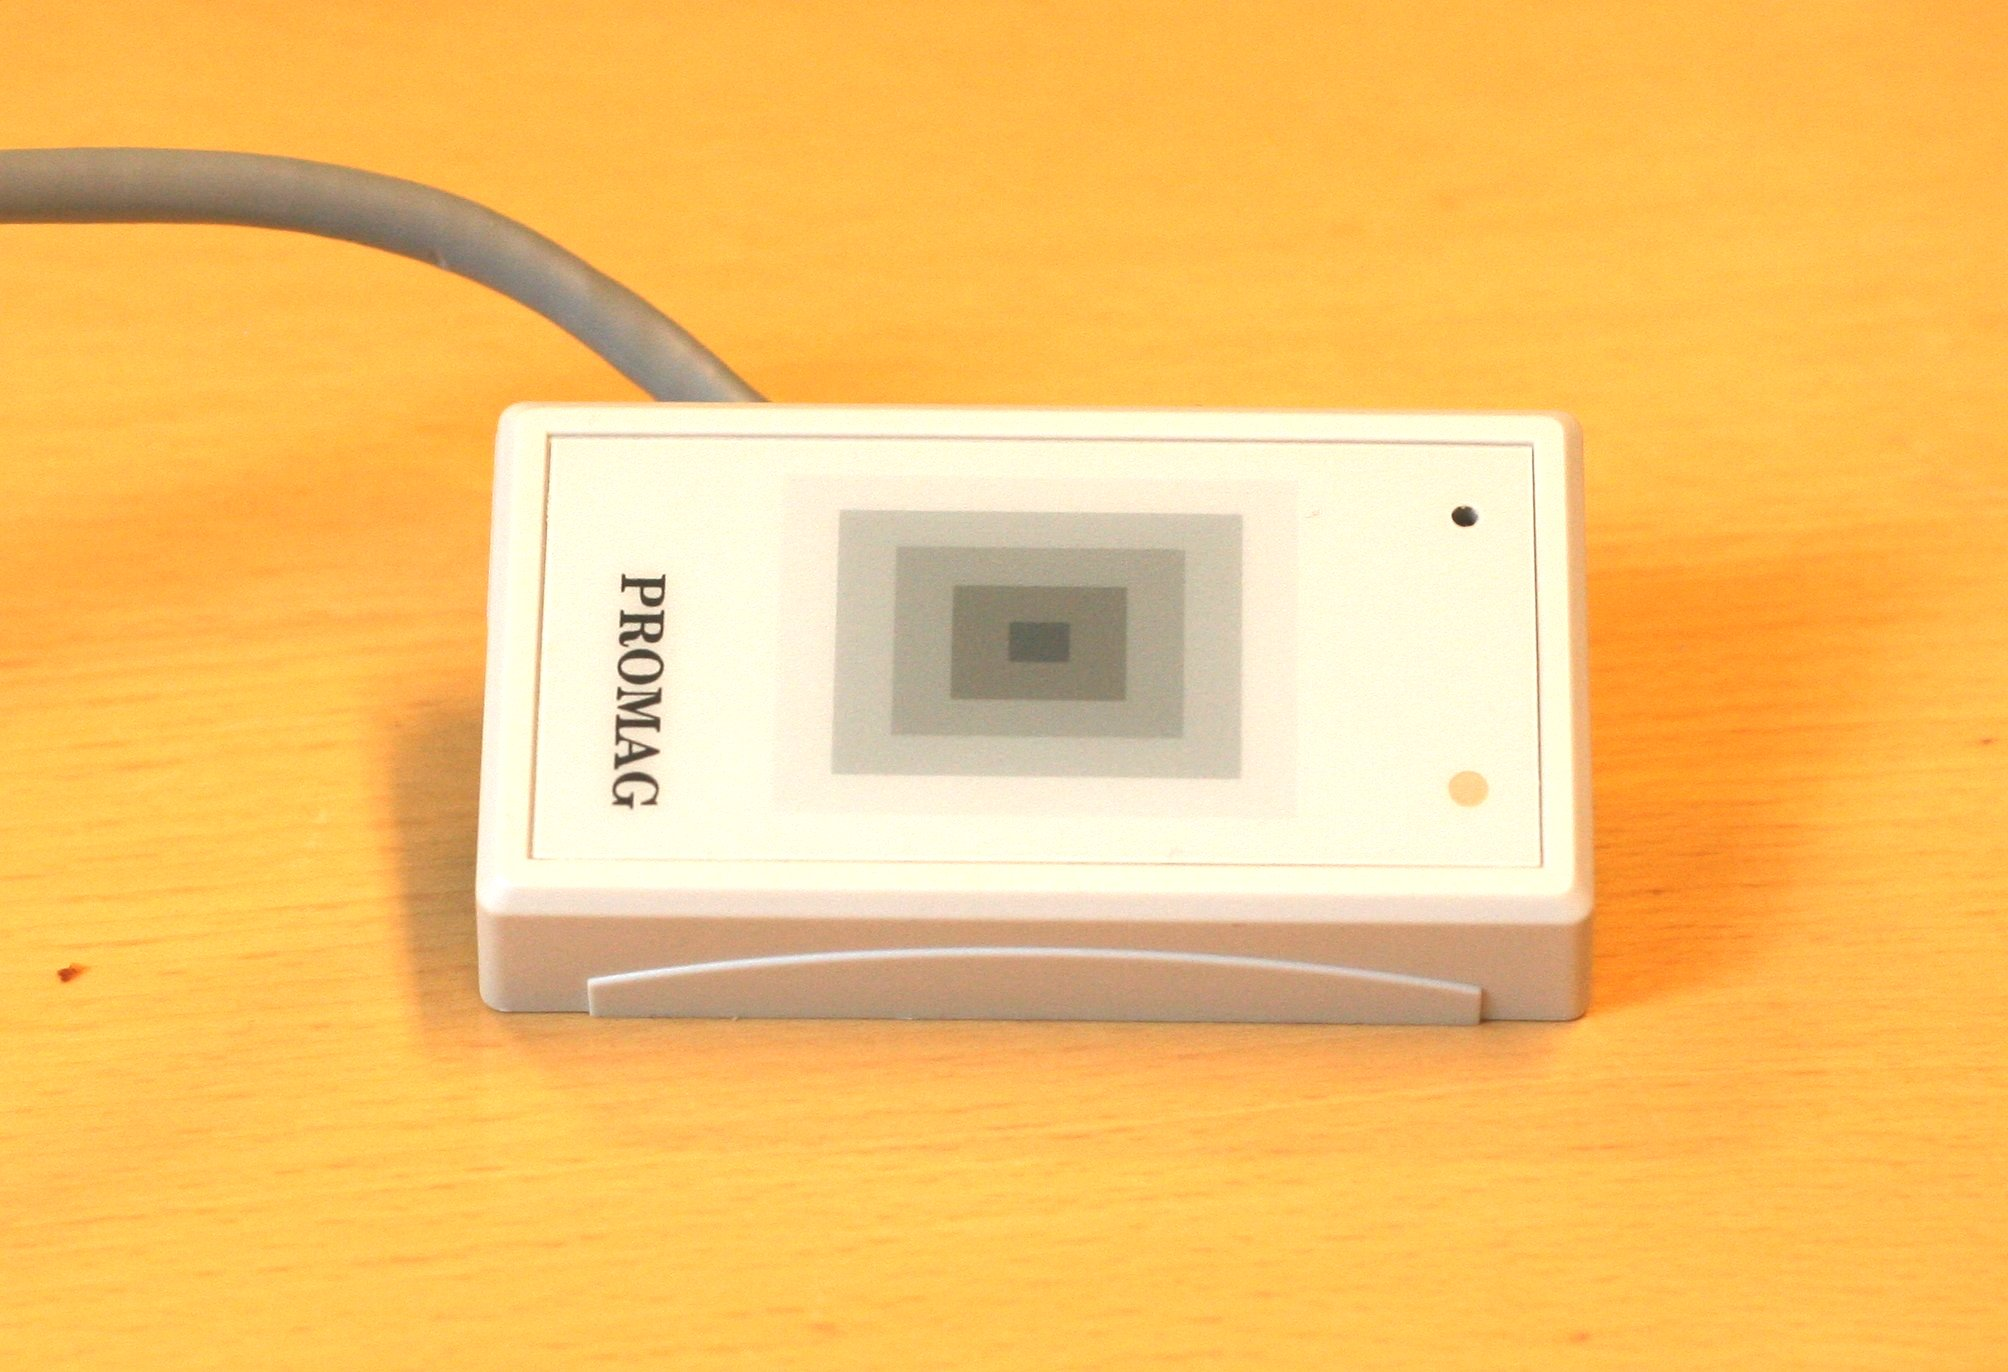
\includegraphics[width=60mm]{antenne_2.eps}
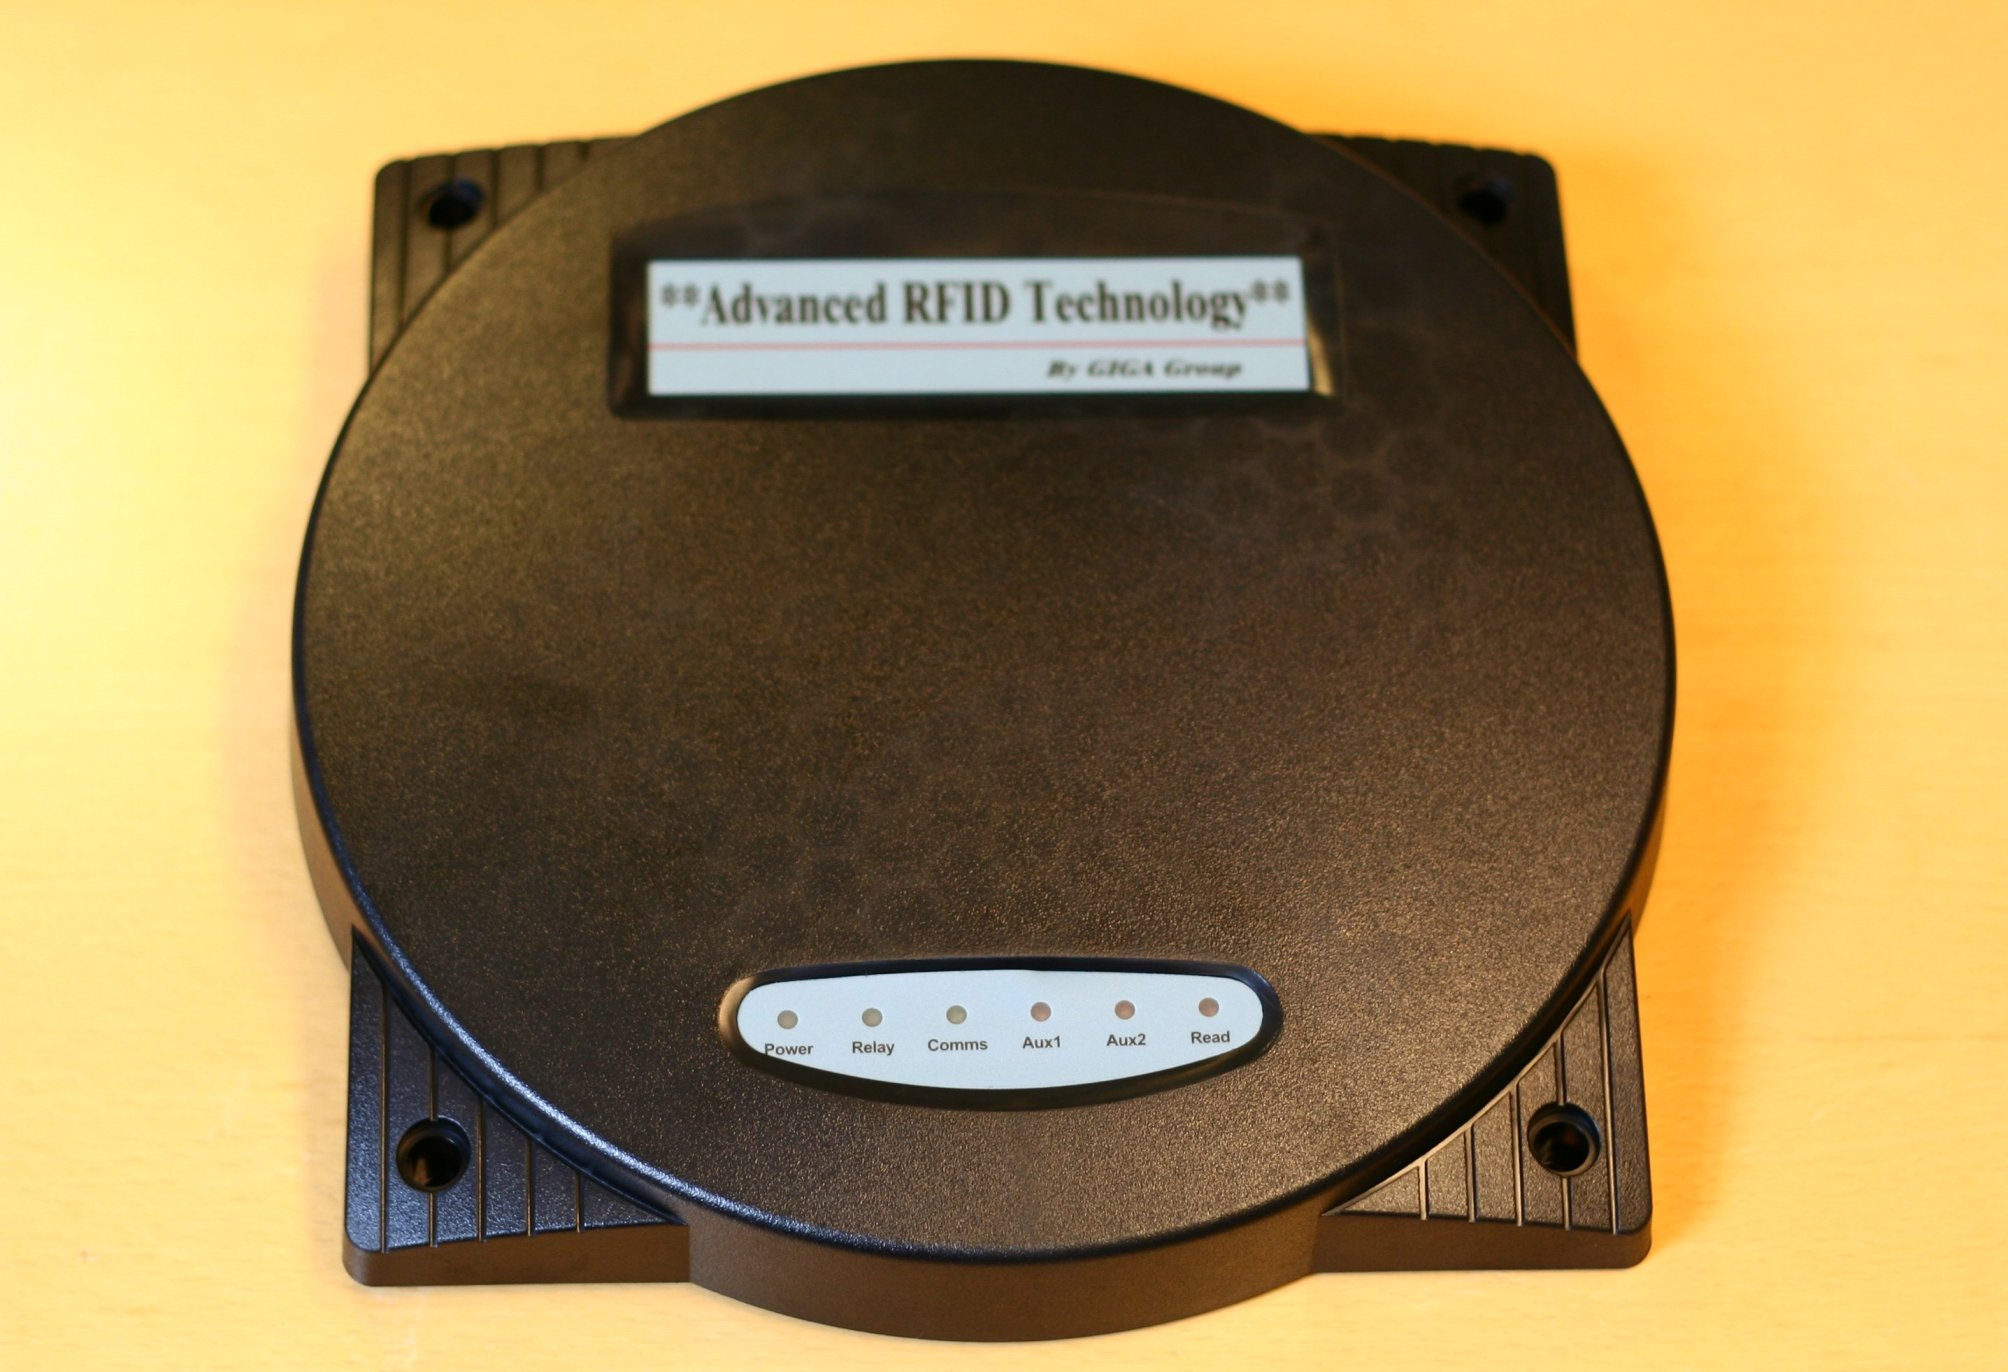
\includegraphics[width=60mm]{antenne_1.eps}\\
\end{center}
\label{antenner}
\caption{De to antenner. Den venstre er den kontinuerlige og den h�jre
  er den ikke kontinuerlige.}
\end{figure}
\begin{figure}
\begin{center}
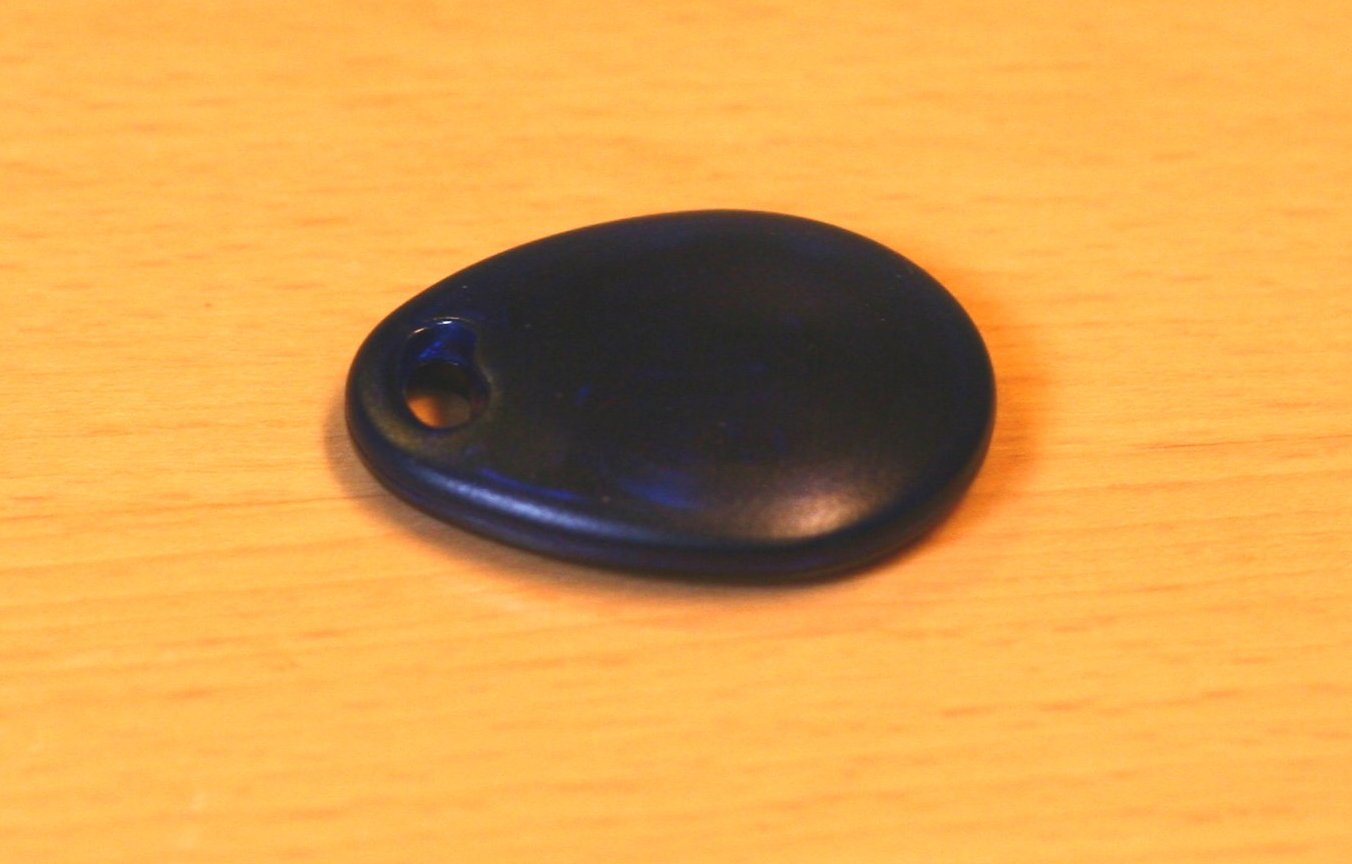
\includegraphics[width=60mm]{transponder_1.eps}
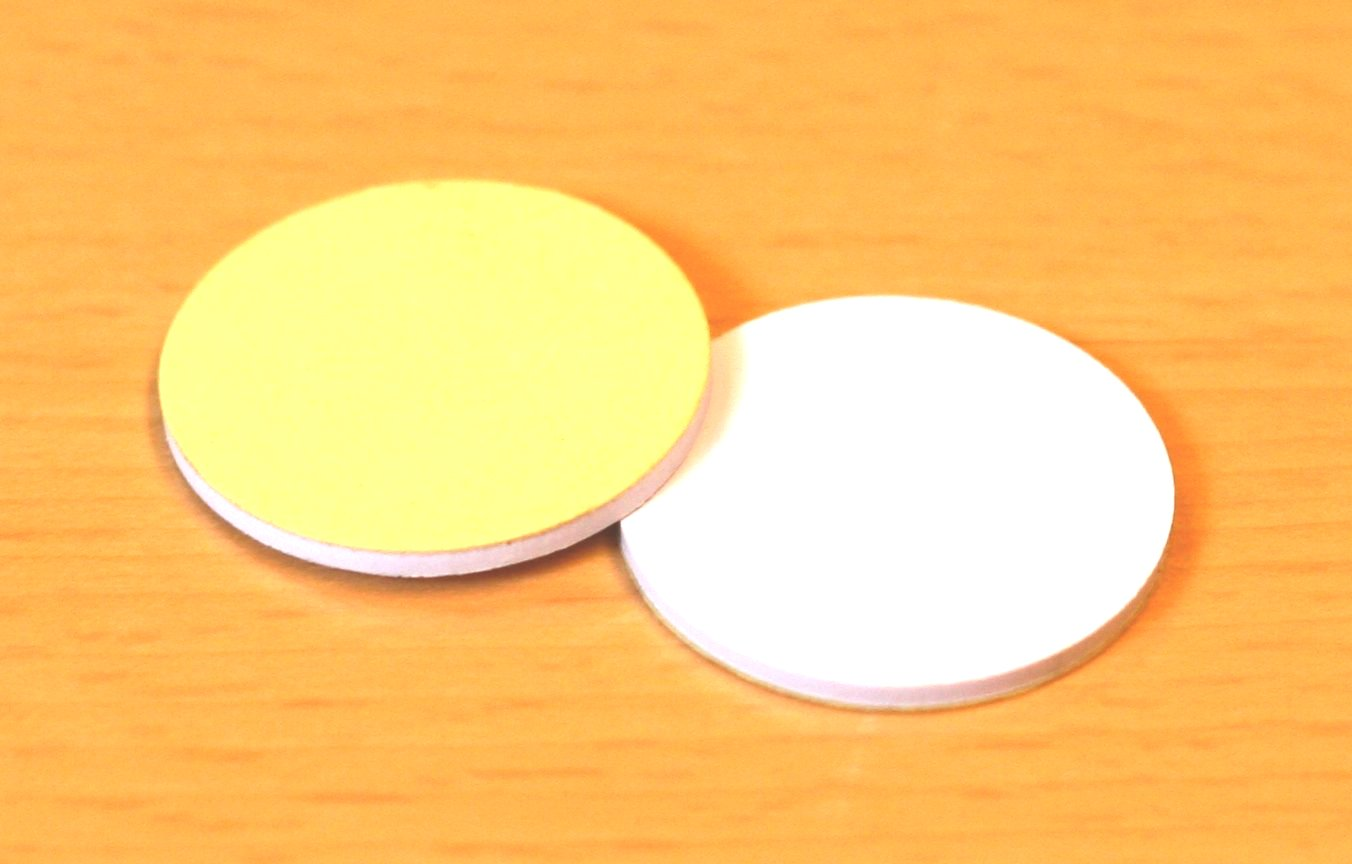
\includegraphics[width=60mm]{transponder_2.eps}\\
\end{center}
\label{transpondere}
\caption{De to transpondertyper. Den venstre er Key transponderen, den
  h�jre er Brick transponderen med tape p� undersiden.}
\end{figure}

\section{Praktiske omst�ndigheder omkring brugen af RFID}
For at en m�ling kan foretages korrekt er det n�dvendigt for systemet
at der er tilknyttet en patient og en operat�r til den givne
lokation.\\
Sammenknytningen skal ske ved at b�de operat�ren og en patienten
registrerer sig i systemet p� lokationen p� samme tid og derved binder
sig sammen i de efterf�lgende m�linger.

\subsection{Operat�ren}
Operat�ren skal opbevare sin transponder p� sig hele tiden mens
systemet benyttes, og det skal derfor laves s� operat�ren ikke bliver
generet af den.\\
N�r en m�ling skal foretages skal operat�ren give sig til kende
overfor sy\-stem\-et vha. sin transponder. Operat�ren skal selv foretage
registreringen, og det forventes at operat�ren f�r god tr�ning i at
benytte systemet, idet det kommer til at blive taget i brug mange
gange dagligt.

\subsection{Patienten}
Patient skal ligesom operat�ren b�re rundt p� en transponder. Den skal
v�re til stede fra patientens ankomst til dagens forl�b er afsluttet.\\
Id�en er at patienten ved ankomst modtager en transponder som internt
i systemet bliver knyttet til patientens stamdata.\\
Alimindeligvis vil det v�re s�dan at patienten selv b�rer rundt p� sin
trans\-pon\-der i lommen eller h�nden, men da visse patienter kan v�re
forhindrede i dette skal det ogs� v�re muligt at b�re den i en snor om
halsen, h�ndledet eller lign.\\
N�r en m�ling skal foretages t�nkes transponderen afleveret til
operat�ren, som skal foretage registreringen.\\
Selve registreringen kan opfattes som kompliceret af udefrakommende og
det kan derfor ikke forventes at patienten selv kan finde foretage
den. Ydermere vil det v�re til stor gene hvis operat�ren ved hver eneste
patient skal til at bruge tid p� at forklare hvordan registreringen
foreg�r.

\subsection{Log ind/ud}
I forbindelse med registrering af patienten kan patientens navn optr�de
p� en sk�rm hvilket fra operat�rens side kan bidrage til den
s�dvanlige dobbelt kontrol af patientientens identitet.\\ 
Det er vigtigt at de m�lte data bliver kyttet til den korrekte
patient i databasen og det b�r derfor g�res s� usandsynligt som muligt
at en uautoriseret m�ling foretages.\\
Et system kan laves som holder styr p� om der b�de er en operat�r og
en patient til stede, samt hvorvidt disse er blevet aktiverede
indenfor en passende tidsramme, f.eks. 30 sekunder.\\
Hvis det ikke er tilf�ldet er systemet i en passiv tilstand hvor det
ikke vil modtage data.\\
Der kan ydermere laves meget nuancerede visuelle repr�sentationer af
sy\-stem\-ets status, s� der aldrig vil opst� tvivl om dette.\\
Dette kan for eksempel g�res ved at lade displayet have en gr� farve
n�r det er passivt, en gr�n n�r det er aktivt og en r�d hvis der er
sket en fejl.\\
Et krav om bekr�ftelse af patientens og operat�rens registrering kan
med fordel tilf�res for at opn� den �nskede sikkerhed for at
operat�ren har foretaget den n�dvendige kontrol. Dette kan eventuelt
implementeres ved hj�lp af en \textit{``bekr�ft''} knap i n�rheden af
antennen.\\
En registrering er aktiv s� l�nge en ny registrering ikke er
foretaget. En log ud knap kan introduceres, som vil efterlade systemet
i passiv tilstand. En timeout p� en registrering er ikke praktisk
mulig idet de forskellige m�linger ikke umidelbart er mulige at s�tte
en �vre tidsgr�nse p�.

\section{Hardware scenarier}
I de f�lgende scenarier bliver f�lgende enheder unders�gt: key
transponder og brick transponder (begge passive read-only), samt en
60cm og en 20cm antenne, hvoraf 20cm antennen er kontinuerlig.\\
Under beskrivelserne vil begrebet \textit{agent} blive benyttet om en
person som b�rer p� en transponder og dermed �nsker at betjene
systemet enten som operat�r eller som patient.

\subsection{Scenarie 1}
\textbf{Hardware:} Key transponder og antenne med en
r�kkevidde p� 60cm.\\

\noindent\textbf{Beskrivelse:} Dette scenarie udarter sig ved at der
er lang aktiveringsafstand mellem transponderen og antennen. Agenten
har transponderen i en n�glering i lommen eller lign. og bliver
automatisk registreret n�r agenten tr�der indenfor et aktiveringfelt,
som er placeret s�dan at man naturligt befinder sig i det n�r man skal
betjene udstyret eller m�les.\\

\noindent\textbf{Fordele:} Agenten kan ikke glemme at logge ind, fordi
agenten �dvendigvis m� befinde sig indenfor aktiveringsomr�det for at
en m�ling kan ofretages.\\
Der skal ikke fortages nogen handling i forbindelse med login og
proceduren er derfor s� simpel og hurtig som det er muligt (med mindre
bekr�ftelse tilf�jes).\\

\noindent\textbf{Ulemper:} Hvis en anden agent bev�ger sig indenfor
aktiveringsomr�det under en m�ling, vil systemet tro at den
oprindelige agent er blevet udskiftet, dette kan dog h�ndteres i
softwaren.\\
Mange apparattyper egner sig ikke til denne type registrering idet det
er sv�rt eller umuligt at definere aktiveringsfeltet.

\subsection{Scenarie 2}
\textbf{Hardware:} Brick transponder og antenne med en
r�kkevidde p� 60cm.\\

\noindent\textbf{Beskrivelse:} I dette scenarie benyttes samme id� som
i scenarie 1, bortset fra at transponderen er udskiftet med en brick
transponder som for eksempel kan v�re monteret p� bagsiden af
navneskiltet (eller noget tilsvarende som agenten altid har p� sig).\\

\noindent\textbf{Fordele:} Alle fordele fra scenarie 1 er ogs� g�ldene
her, men en �ndring er nu at det er nemmere at huske transponderen,
idet den kan placeres p� noget som agenten altid har med sig.\\

\noindent\textbf{Ulemper:} Samme ulemper som ved scenarie 1.\\
Det kan v�re sv�rt at finde noget egnet at montere transponderen p�.

\subsection{Scenarie 3}
\textbf{Hardware:} Key transponder og antenne med en r�kkevidde p�
20cm.\\

\noindent\textbf{Beskrivelse:} I dette scenarie benyttes en
kortr�kkende antenne og en n�g\-le\-rings\-transponder. Transponderen
skal f�res t�t forbi aktiveringsplade for at blive registreret.\\
Antennens mulighed for at l�se kontinuerligt benyttes ikke.\\
Transponderen befinder sig i et n�glebundt i lommen p� agenten eller
lign.\\

\noindent\textbf{Fordele:} Systemet aktiveres ikke fejlagtigt ved en
forbipasserende agent.\\

\noindent\textbf{Ulemper:} Der kr�ves en del interaktion, og det er
nemmere at komme til at glemme at logge ind.

\subsection{Scenarie 4}
\textbf{Hardware:} Key transponder og kontinuerlig antenne med en
r�kkevidde p� 20cm.\\

\noindent\textbf{Beskrivelse:} I dette scenare benyttes samme hardware
som i scenarie 3, men denne gang udnyttes antennens mulighed for at
l�se kontinuerligt.\\
Ved login placerer agenten transponderen i n�rheden af antennen og
lader den ligge der s� l�nge apparatet benyttes.\\

\noindent\textbf{Fordele:} Systemet aktiveres ikke fejlagtigt ved en
forbipasserende agent.\\
Der produceres ekstra informationer om m�lingen, eftersom vi ikke blot
ved hvor\-n�r m�lingen startes foretaget (login) men ogs� hvorn�r den
er slut (n�r transponderen fjernes fra antennen).\\
Log out problemet er s�ledes l�st.\\

\noindent\textbf{Ulemper:} Der kr�ves en del interaktion, og det er
nemt at komme til at glemme at logge ind.\\
Ydermere kan agenten helt glemme at tage transponderen med sig n�r
m�lingen er f�rdig, hvilket vil give anledning til forvirring.

\subsection{Scenarie 5}
\textbf{Hardware:} Brick transponder og kontinuerlig antenne med en
r�kkevidde p� 20cm.\\

\noindent\textbf{Beskrivelse:} Samme scenarie som scenarie 4, bortset
fra at transponderen nu er monteret p� noget som agenten altid har med
sig, men samtidig er villig til at l�gge fra sig.\\

\noindent\textbf{Fordele:} Samme fordele som ved scenarie 4, bortset
fra at det nu er nemmere at huske at logge ind, fordi transponderen er
monteret p� noget som er mere oplagt at l�gge fra sig ved antennen.\\

\noindent\textbf{Ulemper:} Samme fordele som ved scenarie 4, bortset
fra det gerne skulle v�re nemmere at huske at logge ind og nemmere at
huske at tage transponderen med sig ved endt m�ling.\\
Det kan v�re sv�rt at finde et egnet emne at montere tagget p�.

\section{Sikkerhed}
Sikkerheden forbundet med RFID systemet skal ogs� tages i
betragtning.\\
En ondsindet person kan let f� fingre i det tal som transponderen
indeholder, idet han blot kan opstille en antenne tilpads t�t p� den
rigtige antenne (almindeligvis er 1m tilstr�kkelig t�t p�), som kan
l�se tallet.\\
Med tallet i h�nden kan man manuelt kode en anden transponder med
samme tal, hvorved den oprindelige transponder er blevet kopieret.\\
I vores scenarier er det i patientens tilf�lde et sp�rgsm�l om at det
ikke m� kunne lade sig g�re at aflure patientens informationer ved at
l�se det udleverede tag.\\
Dette er h�ndteret ved at det nummer som ligger p� tagget ikke har
nogen direkte forbindelse med patientens stamdata, idet disse kun
ligger p� serveren. Det er s�ledes n�dvendigt for en ondsindet
person ikke blot at tilskaffe sig adgang til patientens tag, men
ogs� til serveren indeholdene stamdataene.\\
Den ondsindede person har s�ledes ikke umiddelbart noget ud af at
kopiere patientens transponder, idet den udl�ber efter et d�gn, og det
eneste han kan opn� er at udgive sig overfor systemet for at v�re den
p�g�ldene patient indenfor det d�gn.\\
Dette vil i v�rste fald give anledning til fejlm�linger som, n�r det
opdages, er nemme af fjerne fra systemet (data ovreskrives aldrig, men
tilf�jes). Samtidig vil det v�re forholdsvis nemt for en operat�r at
opdage.\\
Det er straks mere interressant for den ondsindede person at
kopiere operat�rens transponder, hvilket umiddelbart er lige s� nemt
som at kopiere patientens.\\
Med en operat�rtransponder i h�nden kan den ondsindede person
udgive sig at v�re operat�r overfor systemet og dermed aktivere
uautoriserede m�linger.\\
S�danne uautoriserede m�linger er dog nemme at opdage og eftersom der
ikke slettes eller overskrives data kan de originale data let genskabes.
%Ved en udvidelse af systemet til at h�ndtere
%reelt login til f.eks. PC-Praxis vil det have langt videre r�kkende
%konsekvenser, idet det vil blotte patientf�lsomme data.\\
%Alt dette kan imidlertid modv�rges ved at implementere en s�kaldt
%onetimepad i operat�rens tag, som g�r det umuligt at kopiere ved blot
%at lytte i n�rheden af antennen.\\
Ved ydermere at indf�re en fornuftig politik omkring indrapportering
af stj�lne eller mistede transpondere, vil man g�re det meget sv�rt
for en ondsindet person at f� fat i valide data, idet en forlagt
transponders tal vil bliver erkl�ret ugyldigt forholdsvis hurtigt.

\section{Eksperimenter}
Vi producerede et praktisk testeksempel for at belyse nogle af
uhensigtsm�ssighederne i optillingen.\\
Til form�let blev udviklet en mockup af login softwaren som blev sta
til at k�re p� en touchscreen.\\
Fors�get blev udf�rt i refraktiv kirurgisk afsnit. Operat�ren var Toni
Hansen.\\
F�lgende resultater kom ud af eksperimentet:
\begin{itemize}
\item{Operat�ren puttede transponderen i sin kalender som var
  lokalisret i brystlommen. Ved scanning blev denne s�ledes vist til
  antennen.}
\item{Operat�ren havde brugt RFID teknologi tidligere i forbindelse
  med undergrunds bane rejser.}
\item{Bekr�ftelsen i GUIet skal v�re meget tydelig (specielt
  tydeligere end p� vores mockup)}
\item{Idet patienten blev scannet forholdsvis lang tid inden
  operat�ren, skal der v�re en lang timeout.}
\item{Det afpr�vede ``g� forbi og den aktiveres'' scenarie virkede
  ikke. Antennen var ikke kraftig nok.}
\item{Man skal ``vise'' transponderen til antennen, ikke k�re den
  forbi som man ville g�re det i en stregkodescanner i et supermarked.}
\item{For at undg� dobbelt login kr�ves det at man logger ud hvis man
  allerede er logget ind et andet sted (til gene og derfor kan de
  m�ske huske det!)}
\item{En patient for oftest blot foretaget en enkelt m�ling, sj�ldnere
  sker det at der bliver foretaget 2 eller 3 (NOTE: Specifikt for
  refraktiv).}
\item{Antennen skal monteres p� tr� eller lign. En metalplade (g�lder
  ogs� aluminium) forstyrrer signalet s� meget at systemet n�rmest er
  ubrugeligt.}
\end{itemize}


\part{Design} % Hvordan f�r vi det
\chapter{Software}
Der er i udgangspunkt tre software opgaver som skal l�ses, samt et modul
pr. apparattype der skal kobles op.\\
De tre er:
\begin{itemize}
\item Dataserveren.
\item Soekris boksens software (data indsamling)
\item Klient software (eg. udvidelser til KatBase, PC-Show o. lign.)
\end{itemize}

\section{Overordnet software struktur}
\subsection{Dataserveren}
Dataserveren er den centrale applikation, som kun skal k�re p� \'{e}n
maskine (serveren), men til geng�ld have en meget h�j tilg�ngelighed,
idet den er single point of faliure.\\
Den har tre funktioner:
\begin{itemize}
\item Modtagelse af CPR-numre og data fra Soekris boksene.
\item Kommunikation med databasen (PostgreSQL eller lignende)
\item Besvarelse af foresp�rgsler fra klienterne, derunder
	parsning af r�data.
\end{itemize}
De to �verste opgaver kan laves generisk, idet vi p� disse niveauer
ikke skelner mellem data fra de forskellige apparater.\\
Det sidste punkt kan laves generisk, for hele processen til og med
fortolkningen af dataene. Der skal s�ledes skrives et modul
pr. klienttype samt pr. apparat/data type.\\
Det t�nkes udviklet p� en m�de, s� modulerne let kan tilf�jes
efterh�nden som der bliver koblet mere udstyr p�, uden at skulle f.eks
genstarte serveren.

\begin{center}
\includegraphics[width=120mm]{software.eps}\\
\textit{Figuren viser sammenh�ngen mellem apparater, maskiner, moduler
og datatransport.}
\end{center}

\subsection{Dataindsamling}
Soekris boksens prim�re software skal i udgangspunkt kunne to ting:
Hive data ud fra et apparat (pull) og vente p� data fra et apparat
(push).\\
Disse to opgaver skal fungere vha. af moduler, idet det skal g�res
forskelligt for hver apparattype, der er p� afdelingen. Ligesom p�
serveren t�nkes det udvilket, s� det ikke kr�ver genstart eller
genkompilering af alle applikationerne for at aktivere et nyt modul
(dog skal de maskiner, som skal bruge det nye modul, nok genstartes).\\
N�r en klump data er modtaget fra et apparat skal dette sendes til
dataserveren, sammen med et prekonfigureret lokationsnummer (vi
overvejer at bruge IP-adresserne for at undg� en divergens i boksenes
konfiguration).

\subsection{Klienterne}
Hvad pr�cis der skal laves p� klient omr�det vides endnu ikke, men der
er pt. planer om at udvide KatBase og omskrive PC-Show til brug af det
nye system.
%P� sigt kan det t�nkes at PC-Praxis skal f�lge samme 
%sk�bne, men det afh�nger af en del andre faktorer.\\
Eftersom vi selv har produceret det meste af softwaren
burde det v�re muligt at inddrage alle de klienter, som findes p�
afdelingen i systemet.

\section{Implementation}
\subsection{Modulerne}
For at opn� h�jest mulig generalitet og fleksibilitet overvejes brugen
af et scriptsprog, som compiles og k�res p� runtime. Til r�dighed for
dette scriptsprog skal v�re en r�kke kald til hardwaren p� et lavere
niveau, som giver mulighed for at sende og modtage data fra seriel-
eller USBporten.\\
Et konkret bud p� et scriptsprog som opfylder de ovenn�vnte krav er
LUA (\verb|http://www.lua.org|).

\subsection{Netv�rksprotokoller}
Der kommer prim�rt to typer netv�rkskommunikation p� tale:
Kommunikation mellem Soekris boksene og dataserveren, og
kommunikation mellem dataserveren og klienterne (foresp�rgsler).\\
Derudover skal systemet integreres med den eksisterende CPR-database
til opslag af patientnavne p� baggrund af indtastede CPR-numre.\\

Kommunikationen mellem en Soekrisboks og dataserveren skal indeholde
Soekrisboksens lokationsnummer, en kode som beskriver apparatkilden og
en klump r� data.\\

N�r en transmission er afsendt fra Soekrisboksen, skal serveren svare
med en statuskode, sammen med en status besked, som kan skrives i
loggen p� den p�g�ldene Soekris boks, eller udskrives p� et
display. Dette kan f.eks. v�re navnet p� patienten med det CPR-nummer,
som Soekrisboksen har sendt til serveren, navnet p� linsen med den
stregkode, som er afsendt, eller lignende tekst, som kan benyttes af
brugeren til at verificere det afsendte data. Ved fejl kan teksten med
fordel bruges til at orientere om fejlens art, f.eks. ``Ugyldigt
CPR-nummer.'', eller ``Linsen kunne ikke findes i listen over kendte
linsetyper.''.\\

En klients foresp�rgsel skal indeholde det CPR-nummer, der foresp�rges
p�, den apparatkode der foresp�rges p�, samt en kode eller
formateringsstreng, som beskriver hvordan klienten �nsker at modtage
sit svar.\\

Svaret fra dataserveren til klienten skal indeholde et tidsstempel, som
beskriver, hvorn�r dataene er registrerede, en fejlkode og streng p�
lignende vis som ved svar fra dataserveren til Soekrisboksene, og til
sidst en feltopdelt svarblok, som indeholder de data, som klienten har
forespurgt p�, formateret efter den vedh�ftede formateringsstreng.\\

Al kommunikationen er blokopdelt og varierende i l�ngde og
indhold. Det kr�ves at protokollen er meget fleksibel og let at parse,
hvilket alt sammen peger i retning af XML, idet det er godt til
blokopdelt data af varierende st�rrelse og indhold (det er
selvbeskrivende), og er samtidig et nemt format at h�ndtere ved
parsning, idet der findes en lang r�kke gode v�rkt�jer til at hj�lpe
med netop dette.\\

Kommunikationen mellem dataserveren og alle eksterne servere (SQL, Samba,
CPR, Det Gr�nne System, osv.) vil foreg� via de allerede definerede
protokoller. Konceptuelt er det kun dataserveren, som skal kende til
alle disse, og man kan s�ledes implementere alle eksterne foresp�rgsler
igennem dataserveren, med henblik p� udfasning af gamle systemer.
\chapter{Netv�rk}
Soekrisboksene er koblet op mod dataserveren over det normal
netv�rk, men p� sit eget net og s�ledes isoleret fra
produktionsnettet.

Dette kan g�res ved at s�tte to netkort i dataserveren, som s�ledes
kan modtage apparatdata p� det ene og svare p� foresp�rgsler p� det
andet.

Form�let med at separere nettene er, at vi ikke beh�ver kryptere eller
p� anden vis beskytte de data, som sendes fra apparaterne til
dataserveren. Disse data kan ellers betegnes som f�lsomme data, idet de ofte
vil indeholde f�lsomme personinformationer knyttet sammen med et
CPR-nummer.
Ydermere er det en fordel i forhold til at vedligeholde Soekris
boksene, at nettene er separerede, idet de ikke vil v�re under angreb
fra computervira og lignende.

Nettet skal selvf�lgelig v�re et kabelnet og ikke et tr�dl�st, idet hele
pointen med at det er afsk�rmet og dermed sikkert ellers ville
forsvinde.

Al kommunikation identificeres p� indhold og portnummer, og der skal
s�ledes allokeres faste portnumre til samtlige kommunikationstyper i
systemet.

Da der ikke er tale om store datam�ngder (modsat f.eks MIaV) kan
nettet bygges op af 100MBit enheder.
\chapter{Protokoller}
\section{Server kommunikationsprotokol}
\small
\verbatiminput{../xml/sample.xml}
\normalsize

Dette eksempel illustrerer protokollen som bruges fra klienterne til
serveren, hvad enten det er en data query eller noget data som skal
inds�ttes i serveren.\\

\small
\verbatiminput{../xml/schema.xsd}
\normalsize



\part{Implementation} % Det fik vi
\chapter{�konomi}
Der er fire hovedposter i projektets �konomi. Lokationshardware,
brugerudstyr, serverhardware og s� selvf�lgelig softwareudvikling.\\
De tre f�rste er i her skematiseret i sammenh�ng med deres
enhedspriser.

\section{Udgifter til en lokation}
\begin{tabular}{l l}
Udstyr          & Pris \\
\hline
Soekris boks    & 2000 kr.\\
CPR-indtastning & 1700 kr.\\
RFID l�ser      & 800 kr.\\
PoE (PDS kobling) & 1500 kr.\\
\hline
                & 6000 kr.\\
\end{tabular}

\section{Udgifter pr. bruger}
\begin{tabular}{l l}
Udstyr                     & Pris \\
\hline
RFID kort                  & 30 kr.\\
Personificering af ID kort & ? \\
\hline
                           & $>$ 30 kr.\\
\end{tabular}

\section{Udgifter til server/netv�rk}
\begin{tabular}{l l}
Udstyr           & Pris \\
\hline
Switch, Cisco, 48 porte, managed & 0 kr. (Leveres af IT afdelingen)\\
Server           & 0 kr. (Vi kan bruge en eksisterende)\\
\hline
                 & 0 kr.\\
\end{tabular}

\section{Softwareudvikling}
Det er ikke p� nuv�rende tidpunkt muligt at lave et tidsestimat p�
softwareudviklingen, og dermed heller ikke muligt at lave et prisoverslag.

\appendix
\chapter{Observationer}
\section{Tonometer}
\apparat{Xpert NCT Advanced Logic Tonometer} % Apparat
	{Reichert} % Producent
	{M�ler trykket i �jet} % Form�l
	{Unders�gelsesrum 50} % Placering
	{Lola Gazieva (l�ge)} % Bruger
\begin{itemize}
\item Finder patient i PC-Praxis.
\item Justerer apparatet, s� det rammer i center af det ene �je.
\item Aktivererer m�lingen.
\item Data overf�res automatisk til PC-Praxis.
\item Justerer apparatet, s� det rammer i center af det andet �je.
\item Aktivererer m�lingen.
\item Data overf�res automatisk til PC-Praxis.
\end{itemize}
%%%%%%%%%%%%%%%%%%%%%%%%%%%%%%%%%%%%%%%%%%%%%%%%%%%%%%%%%%%%%%%%%%%%%%%%%%%%%%%
\section{Keratometer}
\apparat{Auto Refraktion Keratometer NRK-8000} % Apparat
	{Nikon} % Producent
	{M�ler den objektive synsstyrke} % Form�l
	{Unders�gelsesrum 50} % Placering
	{Lola Gazieva (l�ge)} % Bruger

\begin{itemize}
\item Finder patient i PC-Praxis.
\item Justerer apparatet, s� det rammer i center af det ene �je.
\item Aktivererer m�lingen.
\item Justerer apparatet, s� det rammer i center af det andet �je.
\item Aktivererer m�lingen.
\item Der trykkes print p� apparatet, og dataene overf�res til PC-Praxis.
\end{itemize}
%%%%%%%%%%%%%%%%%%%%%%%%%%%%%%%%%%%%%%%%%%%%%%%%%%%%%%%%%%%%%%%%%%%%%%%%%%%%%%%
\section{Atlas}
\apparat{Atlas - Corneal Topography System model 995} % Apparat
	{Zeiss} % Producent
	{Laver topologisk kort over hornhinden} % Form�l
	{Unders�gelsesrum 50} % Placering
	{Lola Gazieva (l�ge)} % Bruger
\begin{itemize}
\item Indtaster patienten p� apparatet (apparatet har sin egen database).
\item Justerer apparatet, s� det rammer i center af det ene �je.
\item Aktivererer m�lingen.
\item Justerer apparatet, s� det rammer i center af det andet �je.
\item Aktivererer m�lingen.
\item Der trykkes gem, og de m�lte data lagres p� en lokal disk.
\end{itemize}
%%%%%%%%%%%%%%%%%%%%%%%%%%%%%%%%%%%%%%%%%%%%%%%%%%%%%%%%%%%%%%%%%%%%%%%%%%%%%%%
\section{Phoropter}
\apparat{Visutron Plus} % Apparat
	{MMC} % Producent
	{Finder den subjektive synsstyrke} % Form�l
	{Katerakt spor 1} % Placering
	{Claus S. J�rgensen (l�ge)} % Bruger
\begin{itemize}
\item Patienten sl�s op i KatBase.
%\item Phoropteren rigges til.
\item Phoropteren indstilles til startposition udfra en lap papir fra
	en tidligere udf�rt m�ling (Objektivt synsm�l fra keratometeret).
\item Displayet styres vha. en fjernbetjening (der skrives tal i
	forskellige st�rrelser p� en plade som patienten skal pr�ve at l�se).
\item En linse v�lges vha. kontrolpulten.
\item De to ovenn�vnte skridt gentages til den bedste linse er fundet.
\item Linsernes (begge �jne) karakteristika overf�res til KatBasen
	vha. manuel afl�sing/indtastning.
\end{itemize}
%%%%%%%%%%%%%%%%%%%%%%%%%%%%%%%%%%%%%%%%%%%%%%%%%%%%%%%%%%%%%%%%%%%%%%%%%%%%%%%
\section{Retinomax}
\apparat{Retinomax} % Apparat
	{Nikon} % Producent
	{Transportabelt keratometer. M�ler den objektive synsstyrke} % Form�l
	{Katerakt spor 1. Soklen st�r i hovedunders�glesen} % Placering
	{Claus S. J�rgensen (l�ge)} % Bruger
\begin{itemize}
\item Patienten findes i KatBase.
\item Apparatet flyttes hen til patienten.
\item Apparatet aktiveres, m�ler og lagrer resultatet internt.
\item Apparatet placeres i soklen som er tilsluttet en printer.
\item Der trykkes print og en kassebon kommer ud med resultaterne.
\item Tallene overf�res manuelt (ved indtastning) til KatBase.
\end{itemize}
%%%%%%%%%%%%%%%%%%%%%%%%%%%%%%%%%%%%%%%%%%%%%%%%%%%%%%%%%%%%%%%%%%%%%%%%%%%%%%%
\section{Ultralyd}
\apparat{AL2000 - Ultralyd} % Apparat
	{MMC} % Producent
	{M�ler �jedybden (den invendige l�ngde af �je�blet)} % Form�l
	{Katerakt spor 3} % Placering
	{Martin �vall (l�ge)} % Bruger
\begin{itemize}
\item Patienten sl�s op i KatBase.
\item �jnene dryppes (bed�velse).
\item Ultralydproben monteres p� en spaltelampe for bedre kontrol.
\item Apparatet m�ler kontinuerligt og signalerer om den modtager valid
	data ved et lavfrekvent bip. Den tager 10 m�linger og benytter gennemsnittet heraf. N�r
	komplet data er indsamlet laver den et h�jfrekvent bip.
\item De m�lte resultater printes ved tryk p� print.
\item Nogle af tallene p� det printede indskrives i KatBase.
\item Det printede indscannes, idet det indeholder en graf.
\end{itemize}
%%%%%%%%%%%%%%%%%%%%%%%%%%%%%%%%%%%%%%%%%%%%%%%%%%%%%%%%%%%%%%%%%%%%%%%%%%%%%%%
\section{A4 Scanner}
\apparat{A4 Scanner} % Apparat
	{HP} % Producent
	{Elektronisk lagring af printede/h�ndskrevne dokumenter} % Form�l
	{Katerakt spor 3} % Placering
	{Martin �vall (l�ge)} % Bruger
\begin{itemize}
\item Patienten sl�s op i PC-Praxis.
\item En kategori og et navn indtastes.
\item En genvejstast aktiverer en scanning, som lagres under det
	den aktive patient.
\end{itemize}
%%%%%%%%%%%%%%%%%%%%%%%%%%%%%%%%%%%%%%%%%%%%%%%%%%%%%%%%%%%%%%%%%%%%%%%%%%%%%%%
\section{Spaltelampe}
\apparat{Spaltelampe, inkl. kamera og grabberkort} % Apparat
	{Zeiss} % Producent
	{Tage billeder af skader p� hornhinde og det ydre �je} % Form�l
	{Katerakt spor 1} % Placering
	{Elin Holm (l�ge)} % Bruger
\begin{itemize}
\item Patienten findes i PC-Praxis.
\item PC-Show startes vha. genvejstast i PC-Praxis.
\item PC-Grab startes vha. genvejstast i PC-Show.
\item Der trykkes p� knappen 'T�nd'.
\item Patienten s�ttes til rette og kameraet justeres.
\item N�r det �nskede billede er i spaltelampen, vender l�gen sig om
	mod sk�rmen, og trykker p� knappen 'Frys'.
\item Hvis det aktuelle stilbillede er acceptabelt, trykkes 'Gem'.
\end{itemize}
%%%%%%%%%%%%%%%%%%%%%%%%%%%%%%%%%%%%%%%%%%%%%%%%%%%%%%%%%%%%%%%%%%%%%%%%%%%%%%%
\section{Lensmeter}
\apparat{Lensmeter} % Apparat
	{Humphrey} % Producent
	{M�le styrken af brilleglas} % Form�l
	{Hovedunders�gelse} % Placering
	{Mette Fogedby (sygeplejerske)} % Bruger
\begin{itemize}
\item Det ene brilleglas inds�ttes i apparatet.
\item Der trykkes 'M�l'.
\item Det andet brilleglas inds�ttes i apparatet.
\item Der trykkes 'M�l'.
\item Der trykkes 'Print'.
\item Det printede indscannes.
\item Det printede kasseres.
\end{itemize}
%%%%%%%%%%%%%%%%%%%%%%%%%%%%%%%%%%%%%%%%%%%%%%%%%%%%%%%%%%%%%%%%%%%%%%%%%%%%%%%
\section{Lensmeter}
\apparat{Lensmeter} % Apparat
	{Humphrey} % Producent
	{M�le styrken af brilleglas} % Form�l
	{Hovedunders�gelse} % Placering
	{Tony Hansen (sygeplejerske)} % Bruger
\begin{itemize}
\item Det ene brilleglas inds�ttes i apparatet.
\item Der trykkes 'M�l'.
\item Det andet brilleglas inds�ttes i apparatet.
\item Der trykkes 'M�l'.
\item Der trykkes 'Print'.
\item Det printede indskrives manuelt i PC-Praxis.
\item Det printede kasseres efter et d�gn (gemmes indtil da ved siden af sk�rmen).
\end{itemize}
%%%%%%%%%%%%%%%%%%%%%%%%%%%%%%%%%%%%%%%%%%%%%%%%%%%%%%%%%%%%%%%%%%%%%%%%%%%%%%%
\section{Digitalkamera}
\apparat{Digitalkamera EOS300} % Apparat
	{Canon} % Producent
	{Tage billeder af eksterne �jenskader} % Form�l
	{10A.217} % Placering
	{Steen Urbak (l�ge) og Peter Skaarup (EDB-ansvarlig)} % Bruger
\begin{itemize}
\item Patienten sl�s op i PC-Praxis.
\item Sk�rmen med patientens stamdata vist fotograferes.
\item Der tages billeder af patienten.
\item Kameraet afleveres til den EDB-ansvarlige.
\item Den EDB-ansvarlige l�gger billederne ind i systemet manuelt
	vha. CPR-nummeret fra det billede som blev taget af PC-Praxis
	sk�rmbilledet.
\end{itemize}
%%%%%%%%%%%%%%%%%%%%%%%%%%%%%%%%%%%%%%%%%%%%%%%%%%%%%%%%%%%%%%%%%%%%%%%%%%%%%%%
\section{Pupilometer}
\apparat{Pupilometer P2000 igennem PupilFit} % Apparat
	{Procyon} % Producent
	{M�le st�rrelsen af pupillen under forskellige lysstyrker} % Form�l
	{Unders�gelse 50} % Placering
	{Lene Pedersen (l�ge)} % Bruger
\begin{itemize}
\item Patienten sl�s op i PC-Praxis.
\item Patient oprettes manuelt i PupilFit.
\item Den nyoprettede patient genfindes og v�lges.
\item Der trykkes p� knappen '1'.
\item Der trykkes p� knappen '2'.
\item \textit{A}. Den f�rste lysstyrke v�lges.
\item \textit{B}. Der stilles skarpt.
\item \textit{C}. Der tages billede.
\item \textit{A}, \textit{B} og \textit{C} gentages ved de to andre
	lysstyrker (ikke valgfrit).
\item De producerede data gennemses for fejl.
\item Den producerede gennemsnitsv�rdi for den scotopiske (m�rkeste)
	m�ling afl�ses p� sk�rmen og indtastes i PC-Praxis.
\end{itemize}
%%%%%%%%%%%%%%%%%%%%%%%%%%%%%%%%%%%%%%%%%%%%%%%%%%%%%%%%%%%%%%%%%%%%%%%%%%%%%%%
\section{Ref/Keratometer (mgui)}
\apparat{Ref/Keratometer} % Apparat
	{Nidek} % Producent
	{M�ler den objektive synsstyrke} % Form�l
	{Katerakt spor 3} % Placering
	{Mette Fogedby og Iben Jensen (sygeplejersker)} % Bruger
\begin{itemize}
\item Patientens CPR-nummer indtastes i mgui.
\item Der m�les.
\item Der printes en kassebon med resultaterne.
\item Mgui foresp�rger p� apparatets m�linger, hvorefter disse overf�res.
\item Det printede indscannes og kasseres.
\end{itemize}
%%%%%%%%%%%%%%%%%%%%%%%%%%%%%%%%%%%%%%%%%%%%%%%%%%%%%%%%%%%%%%%%%%%%%%%%%%%%%%%
\section{IOL Master (mgui)}
\apparat{IOL Master} % Apparat
	{Nidek} % Producent
	{M�ler �jets aksel�ngde og kammerdybde, samt hornhindens krumning} % Form�l
	{Katerakt spor 3} % Placering
	{Mette Fogedby og Iben Jensen (sygeplejersker)} % Bruger
\begin{itemize}
\item Patientens CPR-nummer indtastes i mgui.
\item Patienten lokaliseres i apparatet (er blevet overf�rt via mgui).
\item Der m�les.
\item Det m�lte printes ud p� en tilsluttet HP bl�kprinter.
\item Der trykkes p� 'Send' og data overf�res til mgui.
\item Det printede indscannes og kasseres.
\end{itemize}
%%%%%%%%%%%%%%%%%%%%%%%%%%%%%%%%%%%%%%%%%%%%%%%%%%%%%%%%%%%%%%%%%%%%%%%%%%%%%%%
\section{Tonometer (mgui)}
\apparat{Auto non-contact tonometer NT-3000} % Apparat
	{Nidek} % Producent
	{M�ler �jets tryk} % Form�l
	{Katerakt spor 3} % Placering
	{Mette Fogedby og Iben Jensen (sygeplejersker)} % Bruger
\begin{itemize}
\item Patientens CPR-nummer indtastes i mgui.
\item Der m�les.
\item Der printes en kassebon med resultaterne.
\item Mgui foresp�rger p� apparatets m�linger, hvorefter disse overf�res.
\item Det printede indscannes og kasseres.
\end{itemize}
%%%%%%%%%%%%%%%%%%%%%%%%%%%%%%%%%%%%%%%%%%%%%%%%%%%%%%%%%%%%%%%%%%%%%%%%%%%%%%%
\section{Fundus Kamera}
\apparat{Fundus Kamera} % Apparat
	{Canon} % Producent
	{Tager billeder af retina} % Form�l
	{Stue 230} % Placering
	{Vivi Frisk (sygeplejerske)} % Bruger
\begin{itemize}
\item Patienten ankommer og skrives p� en liste (papir).
\item Patienten s�ttes til rette.
\item \textit{A}. Der stilles skarpt.
\item \textit{B}. Der tages billede.
\item \textit{C}. Billedet kontrolleres p� kameraet.
\item Punkterne \textit{A}, \textit{B} og \textit{C} gentages til alle
	de �nskede motiver er produceret.
\item Patientens CPR-nummer indtastes p� computeren.
\item Billederne hentes fra kameraet ved tryk p� 'Hent'.
\item Billederne markeres med �je og position.
\item Der trykkes 'Gem'.
\item Nogle af billederne blev konstateret for m�rke og \textit{A},
	\textit{B}, \textit{C} samt indtastning af CPR-nummeret og sortering gentages
	for at producere nye.
\end{itemize}


%Denne opgave er skrevet ved brug af \LaTeX2e
\end{document}
%*********************************************
%*                 end of                    *
%*              -=DOCUMENT=-                 *
%*********************************************
